
\batchmode
\documentclass[10pt]{amsart}
\usepackage{amsmath,amsfonts,amssymb,multicol}
\usepackage{booktabs,tabularx,colortbl,caption,xcolor}
\usepackage{path}
  \discretionaries |~!@$%^&*()_+`-=#{"}[]:;'<>,.?\/abcdefghijklmnopqrstuvwxyzABCDEFGHIJKLMNOPQRSTUVWXYZ0123456789|
\usepackage[pdftex]{graphicx}
\usepackage{epstopdf}  % allows use of eps files with pdftex
\usepackage{epsf}
\usepackage{epsfig}
\usepackage{pslatex}
\usepackage[utf8]{inputenc}
\pagestyle{plain}
\textheight 9in
\oddsidemargin = -0.42in
\evensidemargin = -0.42in
\textwidth= 7.28in
\columnsep = .25in
\columnseprule = .4pt
\def\endline{\bigskip\hrule width \hsize height 0.8pt }
\newcommand{\lt}{<}
\newcommand{\gt}{>}
\newcommand{\less}{<}
\newcommand{\grt}{>}

% BEGIN capa tex macros

\newcommand{\capa}{{\sl C\kern-.10em\raise-.00ex\hbox{\rm A}\kern-.22em%
{\sl P}\kern-.14em\kern-.01em{\rm A}}}
  
\newenvironment{choicelist}
{\begin{list}{}
	{\setlength{\rightmargin}{0in}\setlength{\leftmargin}{0.13in}
	\setlength{\topsep}{0.05in}\setlength{\itemsep}{0.022in}
	\setlength{\parsep}{0in}\setlength{\belowdisplayskip}{0.04in}
	\setlength{\abovedisplayskip}{0.05in}
	\setlength{\abovedisplayshortskip}{-0.04in}
	\setlength{\belowdisplayshortskip}{0.04in}}
	}
{\end{list}}

% END capa tex macros 

\begin{document}
\voffset=-0.8in
\newpage
\setcounter{page}{1}
\begin{multicols}{2}
\columnwidth=\linewidth
\ifdefined\nocolumns\else \end{multicols}\fi

\noindent {\large \bf  }
\hfill
{\large \bf {Name: \hrulefill ~ Block: \underline{\hspace{1cm}}}}
% Uncomment the line below if this course has sections. Note that this is a comment in TeX mode since this is only processed by LaTeX
%   {\large \bf { Section:  } }
\par
%\par\noindent \bigskip
\noindent{\large \bf {Assignment HomeworkSetFebruary12-February16  due 02/16/2018}}
% Uncomment and edit the line below if this course has a web page. Note that this is a comment in TeX mode.
%See the course web page for information http://yoururl/yourcourse




 \ifdefined\nocolumns\else \begin{multicols}{2}
\columnwidth=\linewidth \fi

\medskip
\goodbreak
\hrule
\nobreak
\smallskip

%%% BEGIN PROBLEM PREAMBLE
{\bf 1.} (1 point) 
%%% END PROBLEM PREAMBLE

Write the sum of \(x+x+x+ 3\) and \(x+x+x+x- 6\) in simplified (standard) form.


\vspace{0.25cm}
\par 
\mbox{\parbox[t]{25ex}{\hrulefill}}



\medskip
\goodbreak
\hrule
\nobreak
\smallskip

%%% BEGIN PROBLEM PREAMBLE
{\bf 2.} (1 point) 
%%% END PROBLEM PREAMBLE
Write the sum of \(x+x+x+ 2\) and \(x+x+x+x+x\) in simplified (standard) form.


\vspace{0.25cm}
\par 
\mbox{\parbox[t]{25ex}{\hrulefill}}



\medskip
\goodbreak
\hrule
\nobreak
\smallskip

    \ifx\pgmlMarker\undefined
      \newdimen\pgmlMarker \pgmlMarker=0.00314159pt  % hack to tell if \newline was used
    \fi
    \ifx\oldnewline\undefined \let\oldnewline=\newline \fi
    \def\newline{\oldnewline\hskip-\pgmlMarker\hskip\pgmlMarker\relax}%
    \parindent=0pt
    \catcode`\^^M=\active
    \def^^M{\ifmmode\else\fi\ignorespaces}%  skip paragraph breaks in the preamble
    \def\par{\ifmmode\else\endgraf\fi\ignorespaces}%
  
%%% BEGIN PROBLEM PREAMBLE
{\bf 3.} (1 point) \ifdim\lastskip=\pgmlMarker
  \let\pgmlPar=\relax
 \else
  \let\pgmlPar=\par
  \vadjust{\kern3pt}%
\fi

%%%%%%%%%%%%%%%%%%%%%%%%%%%%%%%%%%%%%%
%
%    definitions for PGML
%

\ifx\pgmlCount\undefined  % do not redefine if multiple files load PGML.pl
  \newcount\pgmlCount
  \newdimen\pgmlPercent
  \newdimen\pgmlPixels  \pgmlPixels=.5pt
\fi
\pgmlPercent=.01\hsize

\def\pgmlSetup{%
  \parskip=0pt \parindent=0pt
%  \ifdim\lastskip=\pgmlMarker\else\par\fi
  \pgmlPar
}%

\def\pgmlIndent{\par\advance\leftskip by 2em \advance\pgmlPercent by .02em \pgmlCount=0}%
\def\pgmlbulletItem{\par\indent\llap{$\bullet$ }\ignorespaces}%
\def\pgmlcircleItem{\par\indent\llap{$\circ$ }\ignorespaces}%
\def\pgmlsquareItem{\par\indent\llap{\vrule height 1ex width .75ex depth -.25ex\ }\ignorespaces}%
\def\pgmlnumericItem{\par\indent\advance\pgmlCount by 1 \llap{\the\pgmlCount. }\ignorespaces}%
\def\pgmlalphaItem{\par\indent{\advance\pgmlCount by `\a \llap{\char\pgmlCount. }}\advance\pgmlCount by 1\ignorespaces}%
\def\pgmlAlphaItem{\par\indent{\advance\pgmlCount by `\A \llap{\char\pgmlCount. }}\advance\pgmlCount by 1\ignorespaces}%
\def\pgmlromanItem{\par\indent\advance\pgmlCount by 1 \llap{\romannumeral\pgmlCount. }\ignorespaces}%
\def\pgmlRomanItem{\par\indent\advance\pgmlCount by 1 \llap{\uppercase\expandafter{\romannumeral\pgmlCount}. }\ignorespaces}%

\def\pgmlCenter{%
  \par \parfillskip=0pt
  \advance\leftskip by 0pt plus .5\hsize
  \advance\rightskip by 0pt plus .5\hsize
  \def\pgmlBreak{\break}%
}%
\def\pgmlRight{%
  \par \parfillskip=0pt
  \advance\leftskip by 0pt plus \hsize
  \def\pgmlBreak{\break}%
}%

\def\pgmlBreak{\\}%

\def\pgmlHeading#1{%
  \par\bfseries
  \ifcase#1 \or\huge \or\LARGE \or\large \or\normalsize \or\footnotesize \or\scriptsize \fi
}%

\def\pgmlRule#1#2{%
  \par\noindent
  \hbox{%
    \strut%
    \dimen1=\ht\strutbox%
    \advance\dimen1 by -#2%
    \divide\dimen1 by 2%
    \advance\dimen2 by -\dp\strutbox%
    \raise\dimen1\hbox{\vrule width #1 height #2 depth 0pt}%
  }%
  \par
}%

\def\pgmlIC#1{\futurelet\pgmlNext\pgmlCheckIC}%
\def\pgmlCheckIC{\ifx\pgmlNext\pgmlSpace \/\fi}%
{\def\getSpace#1{\global\let\pgmlSpace= }\getSpace{} }%

{\catcode`\ =12\global\let\pgmlSpaceChar= }%
{\obeylines\gdef\pgmlPreformatted{\par\small\ttfamily\hsize=10\hsize\obeyspaces\obeylines\let^^M=\pgmlNL\pgmlNL}}%
\def\pgmlNL{\par\bgroup\catcode`\ =12\pgmlTestSpace}%
\def\pgmlTestSpace{\futurelet\next\pgmlTestChar}%
\def\pgmlTestChar{\ifx\next\pgmlSpaceChar\ \pgmlTestNext\fi\egroup}%
\def\pgmlTestNext\fi\egroup#1{\fi\pgmlTestSpace}%

\def^^M{\ifmmode\else\space\fi\ignorespaces}%
%%%%%%%%%%%%%%%%%%%%%%%%%%%%%%%%%%%%%%

%%% END PROBLEM PREAMBLE
The table below shows the price of movie tickets.

\par 
\par\begin{minipage}{\linewidth}\centering\begin{tabular}{l | c | c | c }\toprule \bfseries  Number of tickets (t) &  3 &  6 &  8 \\\midrule  \bfseries  Price (p) &  \$19.50 &  \$39.00 &  \$52.00 \\\bottomrule\end{tabular}\end{minipage}\par  \vspace{1pc}

Write an equation that can be used to find the price, p, of t tickets.

\vspace{0.25cm}\\
\mbox{\parbox[t]{25ex}{\hrulefill}}



\medskip
\goodbreak
\hrule
\nobreak
\smallskip

%%% BEGIN PROBLEM PREAMBLE
{\bf 4.} (1 point) \ifdim\lastskip=\pgmlMarker
  \let\pgmlPar=\relax
 \else
  \let\pgmlPar=\par
  \vadjust{\kern3pt}%
\fi

%%%%%%%%%%%%%%%%%%%%%%%%%%%%%%%%%%%%%%
%
%    definitions for PGML
%

\ifx\pgmlCount\undefined  % do not redefine if multiple files load PGML.pl
  \newcount\pgmlCount
  \newdimen\pgmlPercent
  \newdimen\pgmlPixels  \pgmlPixels=.5pt
\fi
\pgmlPercent=.01\hsize

\def\pgmlSetup{%
  \parskip=0pt \parindent=0pt
%  \ifdim\lastskip=\pgmlMarker\else\par\fi
  \pgmlPar
}%

\def\pgmlIndent{\par\advance\leftskip by 2em \advance\pgmlPercent by .02em \pgmlCount=0}%
\def\pgmlbulletItem{\par\indent\llap{$\bullet$ }\ignorespaces}%
\def\pgmlcircleItem{\par\indent\llap{$\circ$ }\ignorespaces}%
\def\pgmlsquareItem{\par\indent\llap{\vrule height 1ex width .75ex depth -.25ex\ }\ignorespaces}%
\def\pgmlnumericItem{\par\indent\advance\pgmlCount by 1 \llap{\the\pgmlCount. }\ignorespaces}%
\def\pgmlalphaItem{\par\indent{\advance\pgmlCount by `\a \llap{\char\pgmlCount. }}\advance\pgmlCount by 1\ignorespaces}%
\def\pgmlAlphaItem{\par\indent{\advance\pgmlCount by `\A \llap{\char\pgmlCount. }}\advance\pgmlCount by 1\ignorespaces}%
\def\pgmlromanItem{\par\indent\advance\pgmlCount by 1 \llap{\romannumeral\pgmlCount. }\ignorespaces}%
\def\pgmlRomanItem{\par\indent\advance\pgmlCount by 1 \llap{\uppercase\expandafter{\romannumeral\pgmlCount}. }\ignorespaces}%

\def\pgmlCenter{%
  \par \parfillskip=0pt
  \advance\leftskip by 0pt plus .5\hsize
  \advance\rightskip by 0pt plus .5\hsize
  \def\pgmlBreak{\break}%
}%
\def\pgmlRight{%
  \par \parfillskip=0pt
  \advance\leftskip by 0pt plus \hsize
  \def\pgmlBreak{\break}%
}%

\def\pgmlBreak{\\}%

\def\pgmlHeading#1{%
  \par\bfseries
  \ifcase#1 \or\huge \or\LARGE \or\large \or\normalsize \or\footnotesize \or\scriptsize \fi
}%

\def\pgmlRule#1#2{%
  \par\noindent
  \hbox{%
    \strut%
    \dimen1=\ht\strutbox%
    \advance\dimen1 by -#2%
    \divide\dimen1 by 2%
    \advance\dimen2 by -\dp\strutbox%
    \raise\dimen1\hbox{\vrule width #1 height #2 depth 0pt}%
  }%
  \par
}%

\def\pgmlIC#1{\futurelet\pgmlNext\pgmlCheckIC}%
\def\pgmlCheckIC{\ifx\pgmlNext\pgmlSpace \/\fi}%
{\def\getSpace#1{\global\let\pgmlSpace= }\getSpace{} }%

{\catcode`\ =12\global\let\pgmlSpaceChar= }%
{\obeylines\gdef\pgmlPreformatted{\par\small\ttfamily\hsize=10\hsize\obeyspaces\obeylines\let^^M=\pgmlNL\pgmlNL}}%
\def\pgmlNL{\par\bgroup\catcode`\ =12\pgmlTestSpace}%
\def\pgmlTestSpace{\futurelet\next\pgmlTestChar}%
\def\pgmlTestChar{\ifx\next\pgmlSpaceChar\ \pgmlTestNext\fi\egroup}%
\def\pgmlTestNext\fi\egroup#1{\fi\pgmlTestSpace}%

\def^^M{\ifmmode\else\space\fi\ignorespaces}%
%%%%%%%%%%%%%%%%%%%%%%%%%%%%%%%%%%%%%%

%%% END PROBLEM PREAMBLE
Simplify

\vspace{0.25cm}
\par 
\(-7 x + (-6 x) + 7 x\)= \mbox{\parbox[t]{25ex}{\hrulefill}}



\medskip
\goodbreak
\hrule
\nobreak
\smallskip

%%% BEGIN PROBLEM PREAMBLE
{\bf 5.} (1 point) \ifdim\lastskip=\pgmlMarker
  \let\pgmlPar=\relax
 \else
  \let\pgmlPar=\par
  \vadjust{\kern3pt}%
\fi

%%%%%%%%%%%%%%%%%%%%%%%%%%%%%%%%%%%%%%
%
%    definitions for PGML
%

\ifx\pgmlCount\undefined  % do not redefine if multiple files load PGML.pl
  \newcount\pgmlCount
  \newdimen\pgmlPercent
  \newdimen\pgmlPixels  \pgmlPixels=.5pt
\fi
\pgmlPercent=.01\hsize

\def\pgmlSetup{%
  \parskip=0pt \parindent=0pt
%  \ifdim\lastskip=\pgmlMarker\else\par\fi
  \pgmlPar
}%

\def\pgmlIndent{\par\advance\leftskip by 2em \advance\pgmlPercent by .02em \pgmlCount=0}%
\def\pgmlbulletItem{\par\indent\llap{$\bullet$ }\ignorespaces}%
\def\pgmlcircleItem{\par\indent\llap{$\circ$ }\ignorespaces}%
\def\pgmlsquareItem{\par\indent\llap{\vrule height 1ex width .75ex depth -.25ex\ }\ignorespaces}%
\def\pgmlnumericItem{\par\indent\advance\pgmlCount by 1 \llap{\the\pgmlCount. }\ignorespaces}%
\def\pgmlalphaItem{\par\indent{\advance\pgmlCount by `\a \llap{\char\pgmlCount. }}\advance\pgmlCount by 1\ignorespaces}%
\def\pgmlAlphaItem{\par\indent{\advance\pgmlCount by `\A \llap{\char\pgmlCount. }}\advance\pgmlCount by 1\ignorespaces}%
\def\pgmlromanItem{\par\indent\advance\pgmlCount by 1 \llap{\romannumeral\pgmlCount. }\ignorespaces}%
\def\pgmlRomanItem{\par\indent\advance\pgmlCount by 1 \llap{\uppercase\expandafter{\romannumeral\pgmlCount}. }\ignorespaces}%

\def\pgmlCenter{%
  \par \parfillskip=0pt
  \advance\leftskip by 0pt plus .5\hsize
  \advance\rightskip by 0pt plus .5\hsize
  \def\pgmlBreak{\break}%
}%
\def\pgmlRight{%
  \par \parfillskip=0pt
  \advance\leftskip by 0pt plus \hsize
  \def\pgmlBreak{\break}%
}%

\def\pgmlBreak{\\}%

\def\pgmlHeading#1{%
  \par\bfseries
  \ifcase#1 \or\huge \or\LARGE \or\large \or\normalsize \or\footnotesize \or\scriptsize \fi
}%

\def\pgmlRule#1#2{%
  \par\noindent
  \hbox{%
    \strut%
    \dimen1=\ht\strutbox%
    \advance\dimen1 by -#2%
    \divide\dimen1 by 2%
    \advance\dimen2 by -\dp\strutbox%
    \raise\dimen1\hbox{\vrule width #1 height #2 depth 0pt}%
  }%
  \par
}%

\def\pgmlIC#1{\futurelet\pgmlNext\pgmlCheckIC}%
\def\pgmlCheckIC{\ifx\pgmlNext\pgmlSpace \/\fi}%
{\def\getSpace#1{\global\let\pgmlSpace= }\getSpace{} }%

{\catcode`\ =12\global\let\pgmlSpaceChar= }%
{\obeylines\gdef\pgmlPreformatted{\par\small\ttfamily\hsize=10\hsize\obeyspaces\obeylines\let^^M=\pgmlNL\pgmlNL}}%
\def\pgmlNL{\par\bgroup\catcode`\ =12\pgmlTestSpace}%
\def\pgmlTestSpace{\futurelet\next\pgmlTestChar}%
\def\pgmlTestChar{\ifx\next\pgmlSpaceChar\ \pgmlTestNext\fi\egroup}%
\def\pgmlTestNext\fi\egroup#1{\fi\pgmlTestSpace}%

\def^^M{\ifmmode\else\space\fi\ignorespaces}%
%%%%%%%%%%%%%%%%%%%%%%%%%%%%%%%%%%%%%%

%%% END PROBLEM PREAMBLE
Pat cleans windows during the summer. He
charges \$50 per house and an additional \$5 per
window. Write an expression to represent how much
Pat would charge to clean \(x\) windows at 1 house.

\par 
\mbox{\parbox[t]{25ex}{\hrulefill}}



\medskip
\goodbreak
\hrule
\nobreak
\smallskip

%%% BEGIN PROBLEM PREAMBLE
{\bf 6.} (1 point) \ifdim\lastskip=\pgmlMarker
  \let\pgmlPar=\relax
 \else
  \let\pgmlPar=\par
  \vadjust{\kern3pt}%
\fi

%%%%%%%%%%%%%%%%%%%%%%%%%%%%%%%%%%%%%%
%
%    definitions for PGML
%

\ifx\pgmlCount\undefined  % do not redefine if multiple files load PGML.pl
  \newcount\pgmlCount
  \newdimen\pgmlPercent
  \newdimen\pgmlPixels  \pgmlPixels=.5pt
\fi
\pgmlPercent=.01\hsize

\def\pgmlSetup{%
  \parskip=0pt \parindent=0pt
%  \ifdim\lastskip=\pgmlMarker\else\par\fi
  \pgmlPar
}%

\def\pgmlIndent{\par\advance\leftskip by 2em \advance\pgmlPercent by .02em \pgmlCount=0}%
\def\pgmlbulletItem{\par\indent\llap{$\bullet$ }\ignorespaces}%
\def\pgmlcircleItem{\par\indent\llap{$\circ$ }\ignorespaces}%
\def\pgmlsquareItem{\par\indent\llap{\vrule height 1ex width .75ex depth -.25ex\ }\ignorespaces}%
\def\pgmlnumericItem{\par\indent\advance\pgmlCount by 1 \llap{\the\pgmlCount. }\ignorespaces}%
\def\pgmlalphaItem{\par\indent{\advance\pgmlCount by `\a \llap{\char\pgmlCount. }}\advance\pgmlCount by 1\ignorespaces}%
\def\pgmlAlphaItem{\par\indent{\advance\pgmlCount by `\A \llap{\char\pgmlCount. }}\advance\pgmlCount by 1\ignorespaces}%
\def\pgmlromanItem{\par\indent\advance\pgmlCount by 1 \llap{\romannumeral\pgmlCount. }\ignorespaces}%
\def\pgmlRomanItem{\par\indent\advance\pgmlCount by 1 \llap{\uppercase\expandafter{\romannumeral\pgmlCount}. }\ignorespaces}%

\def\pgmlCenter{%
  \par \parfillskip=0pt
  \advance\leftskip by 0pt plus .5\hsize
  \advance\rightskip by 0pt plus .5\hsize
  \def\pgmlBreak{\break}%
}%
\def\pgmlRight{%
  \par \parfillskip=0pt
  \advance\leftskip by 0pt plus \hsize
  \def\pgmlBreak{\break}%
}%

\def\pgmlBreak{\\}%

\def\pgmlHeading#1{%
  \par\bfseries
  \ifcase#1 \or\huge \or\LARGE \or\large \or\normalsize \or\footnotesize \or\scriptsize \fi
}%

\def\pgmlRule#1#2{%
  \par\noindent
  \hbox{%
    \strut%
    \dimen1=\ht\strutbox%
    \advance\dimen1 by -#2%
    \divide\dimen1 by 2%
    \advance\dimen2 by -\dp\strutbox%
    \raise\dimen1\hbox{\vrule width #1 height #2 depth 0pt}%
  }%
  \par
}%

\def\pgmlIC#1{\futurelet\pgmlNext\pgmlCheckIC}%
\def\pgmlCheckIC{\ifx\pgmlNext\pgmlSpace \/\fi}%
{\def\getSpace#1{\global\let\pgmlSpace= }\getSpace{} }%

{\catcode`\ =12\global\let\pgmlSpaceChar= }%
{\obeylines\gdef\pgmlPreformatted{\par\small\ttfamily\hsize=10\hsize\obeyspaces\obeylines\let^^M=\pgmlNL\pgmlNL}}%
\def\pgmlNL{\par\bgroup\catcode`\ =12\pgmlTestSpace}%
\def\pgmlTestSpace{\futurelet\next\pgmlTestChar}%
\def\pgmlTestChar{\ifx\next\pgmlSpaceChar\ \pgmlTestNext\fi\egroup}%
\def\pgmlTestNext\fi\egroup#1{\fi\pgmlTestSpace}%

\def^^M{\ifmmode\else\space\fi\ignorespaces}%
%%%%%%%%%%%%%%%%%%%%%%%%%%%%%%%%%%%%%%

%%% END PROBLEM PREAMBLE
Simplify

\vspace{0.25cm}
\par 
\(4 (9 x) + 2 y (2) =\) \mbox{\parbox[t]{25ex}{\hrulefill}}

\vspace{0.25cm}
\par 
\(2 \cdot 5 z =\) \mbox{\parbox[t]{25ex}{\hrulefill}}

\vspace{0.25cm}
\par 
\(4 (9 x) + 2 y (2) + 2 \cdot 5 z =\) \mbox{\parbox[t]{25ex}{\hrulefill}}



\medskip
\goodbreak
\hrule
\nobreak
\smallskip

%%% BEGIN PROBLEM PREAMBLE
{\bf 7.} (1 point) \ifdim\lastskip=\pgmlMarker
  \let\pgmlPar=\relax
 \else
  \let\pgmlPar=\par
  \vadjust{\kern3pt}%
\fi

%%%%%%%%%%%%%%%%%%%%%%%%%%%%%%%%%%%%%%
%
%    definitions for PGML
%

\ifx\pgmlCount\undefined  % do not redefine if multiple files load PGML.pl
  \newcount\pgmlCount
  \newdimen\pgmlPercent
  \newdimen\pgmlPixels  \pgmlPixels=.5pt
\fi
\pgmlPercent=.01\hsize

\def\pgmlSetup{%
  \parskip=0pt \parindent=0pt
%  \ifdim\lastskip=\pgmlMarker\else\par\fi
  \pgmlPar
}%

\def\pgmlIndent{\par\advance\leftskip by 2em \advance\pgmlPercent by .02em \pgmlCount=0}%
\def\pgmlbulletItem{\par\indent\llap{$\bullet$ }\ignorespaces}%
\def\pgmlcircleItem{\par\indent\llap{$\circ$ }\ignorespaces}%
\def\pgmlsquareItem{\par\indent\llap{\vrule height 1ex width .75ex depth -.25ex\ }\ignorespaces}%
\def\pgmlnumericItem{\par\indent\advance\pgmlCount by 1 \llap{\the\pgmlCount. }\ignorespaces}%
\def\pgmlalphaItem{\par\indent{\advance\pgmlCount by `\a \llap{\char\pgmlCount. }}\advance\pgmlCount by 1\ignorespaces}%
\def\pgmlAlphaItem{\par\indent{\advance\pgmlCount by `\A \llap{\char\pgmlCount. }}\advance\pgmlCount by 1\ignorespaces}%
\def\pgmlromanItem{\par\indent\advance\pgmlCount by 1 \llap{\romannumeral\pgmlCount. }\ignorespaces}%
\def\pgmlRomanItem{\par\indent\advance\pgmlCount by 1 \llap{\uppercase\expandafter{\romannumeral\pgmlCount}. }\ignorespaces}%

\def\pgmlCenter{%
  \par \parfillskip=0pt
  \advance\leftskip by 0pt plus .5\hsize
  \advance\rightskip by 0pt plus .5\hsize
  \def\pgmlBreak{\break}%
}%
\def\pgmlRight{%
  \par \parfillskip=0pt
  \advance\leftskip by 0pt plus \hsize
  \def\pgmlBreak{\break}%
}%

\def\pgmlBreak{\\}%

\def\pgmlHeading#1{%
  \par\bfseries
  \ifcase#1 \or\huge \or\LARGE \or\large \or\normalsize \or\footnotesize \or\scriptsize \fi
}%

\def\pgmlRule#1#2{%
  \par\noindent
  \hbox{%
    \strut%
    \dimen1=\ht\strutbox%
    \advance\dimen1 by -#2%
    \divide\dimen1 by 2%
    \advance\dimen2 by -\dp\strutbox%
    \raise\dimen1\hbox{\vrule width #1 height #2 depth 0pt}%
  }%
  \par
}%

\def\pgmlIC#1{\futurelet\pgmlNext\pgmlCheckIC}%
\def\pgmlCheckIC{\ifx\pgmlNext\pgmlSpace \/\fi}%
{\def\getSpace#1{\global\let\pgmlSpace= }\getSpace{} }%

{\catcode`\ =12\global\let\pgmlSpaceChar= }%
{\obeylines\gdef\pgmlPreformatted{\par\small\ttfamily\hsize=10\hsize\obeyspaces\obeylines\let^^M=\pgmlNL\pgmlNL}}%
\def\pgmlNL{\par\bgroup\catcode`\ =12\pgmlTestSpace}%
\def\pgmlTestSpace{\futurelet\next\pgmlTestChar}%
\def\pgmlTestChar{\ifx\next\pgmlSpaceChar\ \pgmlTestNext\fi\egroup}%
\def\pgmlTestNext\fi\egroup#1{\fi\pgmlTestSpace}%

\def^^M{\ifmmode\else\space\fi\ignorespaces}%
%%%%%%%%%%%%%%%%%%%%%%%%%%%%%%%%%%%%%%

%%% END PROBLEM PREAMBLE
Simplify


\vspace{0.25cm}
\par 
\(2 b -(8 b -3)\)= \mbox{\parbox[t]{25ex}{\hrulefill}}



\medskip
\goodbreak
\hrule
\nobreak
\smallskip

%%% BEGIN PROBLEM PREAMBLE
{\bf 8.} (1 point) \ifdim\lastskip=\pgmlMarker
  \let\pgmlPar=\relax
 \else
  \let\pgmlPar=\par
  \vadjust{\kern3pt}%
\fi

%%%%%%%%%%%%%%%%%%%%%%%%%%%%%%%%%%%%%%
%
%    definitions for PGML
%

\ifx\pgmlCount\undefined  % do not redefine if multiple files load PGML.pl
  \newcount\pgmlCount
  \newdimen\pgmlPercent
  \newdimen\pgmlPixels  \pgmlPixels=.5pt
\fi
\pgmlPercent=.01\hsize

\def\pgmlSetup{%
  \parskip=0pt \parindent=0pt
%  \ifdim\lastskip=\pgmlMarker\else\par\fi
  \pgmlPar
}%

\def\pgmlIndent{\par\advance\leftskip by 2em \advance\pgmlPercent by .02em \pgmlCount=0}%
\def\pgmlbulletItem{\par\indent\llap{$\bullet$ }\ignorespaces}%
\def\pgmlcircleItem{\par\indent\llap{$\circ$ }\ignorespaces}%
\def\pgmlsquareItem{\par\indent\llap{\vrule height 1ex width .75ex depth -.25ex\ }\ignorespaces}%
\def\pgmlnumericItem{\par\indent\advance\pgmlCount by 1 \llap{\the\pgmlCount. }\ignorespaces}%
\def\pgmlalphaItem{\par\indent{\advance\pgmlCount by `\a \llap{\char\pgmlCount. }}\advance\pgmlCount by 1\ignorespaces}%
\def\pgmlAlphaItem{\par\indent{\advance\pgmlCount by `\A \llap{\char\pgmlCount. }}\advance\pgmlCount by 1\ignorespaces}%
\def\pgmlromanItem{\par\indent\advance\pgmlCount by 1 \llap{\romannumeral\pgmlCount. }\ignorespaces}%
\def\pgmlRomanItem{\par\indent\advance\pgmlCount by 1 \llap{\uppercase\expandafter{\romannumeral\pgmlCount}. }\ignorespaces}%

\def\pgmlCenter{%
  \par \parfillskip=0pt
  \advance\leftskip by 0pt plus .5\hsize
  \advance\rightskip by 0pt plus .5\hsize
  \def\pgmlBreak{\break}%
}%
\def\pgmlRight{%
  \par \parfillskip=0pt
  \advance\leftskip by 0pt plus \hsize
  \def\pgmlBreak{\break}%
}%

\def\pgmlBreak{\\}%

\def\pgmlHeading#1{%
  \par\bfseries
  \ifcase#1 \or\huge \or\LARGE \or\large \or\normalsize \or\footnotesize \or\scriptsize \fi
}%

\def\pgmlRule#1#2{%
  \par\noindent
  \hbox{%
    \strut%
    \dimen1=\ht\strutbox%
    \advance\dimen1 by -#2%
    \divide\dimen1 by 2%
    \advance\dimen2 by -\dp\strutbox%
    \raise\dimen1\hbox{\vrule width #1 height #2 depth 0pt}%
  }%
  \par
}%

\def\pgmlIC#1{\futurelet\pgmlNext\pgmlCheckIC}%
\def\pgmlCheckIC{\ifx\pgmlNext\pgmlSpace \/\fi}%
{\def\getSpace#1{\global\let\pgmlSpace= }\getSpace{} }%

{\catcode`\ =12\global\let\pgmlSpaceChar= }%
{\obeylines\gdef\pgmlPreformatted{\par\small\ttfamily\hsize=10\hsize\obeyspaces\obeylines\let^^M=\pgmlNL\pgmlNL}}%
\def\pgmlNL{\par\bgroup\catcode`\ =12\pgmlTestSpace}%
\def\pgmlTestSpace{\futurelet\next\pgmlTestChar}%
\def\pgmlTestChar{\ifx\next\pgmlSpaceChar\ \pgmlTestNext\fi\egroup}%
\def\pgmlTestNext\fi\egroup#1{\fi\pgmlTestSpace}%

\def^^M{\ifmmode\else\space\fi\ignorespaces}%
%%%%%%%%%%%%%%%%%%%%%%%%%%%%%%%%%%%%%%

%%% END PROBLEM PREAMBLE
Simplify


\vspace{0.25cm}
\par 
\(7 + 4(5 + w)\)= \mbox{\parbox[t]{25ex}{\hrulefill}}



\medskip
\goodbreak
\hrule
\nobreak
\smallskip

%%% BEGIN PROBLEM PREAMBLE
{\bf 9.} (1 point) \ifdim\lastskip=\pgmlMarker
  \let\pgmlPar=\relax
 \else
  \let\pgmlPar=\par
  \vadjust{\kern3pt}%
\fi

%%%%%%%%%%%%%%%%%%%%%%%%%%%%%%%%%%%%%%
%
%    definitions for PGML
%

\ifx\pgmlCount\undefined  % do not redefine if multiple files load PGML.pl
  \newcount\pgmlCount
  \newdimen\pgmlPercent
  \newdimen\pgmlPixels  \pgmlPixels=.5pt
\fi
\pgmlPercent=.01\hsize

\def\pgmlSetup{%
  \parskip=0pt \parindent=0pt
%  \ifdim\lastskip=\pgmlMarker\else\par\fi
  \pgmlPar
}%

\def\pgmlIndent{\par\advance\leftskip by 2em \advance\pgmlPercent by .02em \pgmlCount=0}%
\def\pgmlbulletItem{\par\indent\llap{$\bullet$ }\ignorespaces}%
\def\pgmlcircleItem{\par\indent\llap{$\circ$ }\ignorespaces}%
\def\pgmlsquareItem{\par\indent\llap{\vrule height 1ex width .75ex depth -.25ex\ }\ignorespaces}%
\def\pgmlnumericItem{\par\indent\advance\pgmlCount by 1 \llap{\the\pgmlCount. }\ignorespaces}%
\def\pgmlalphaItem{\par\indent{\advance\pgmlCount by `\a \llap{\char\pgmlCount. }}\advance\pgmlCount by 1\ignorespaces}%
\def\pgmlAlphaItem{\par\indent{\advance\pgmlCount by `\A \llap{\char\pgmlCount. }}\advance\pgmlCount by 1\ignorespaces}%
\def\pgmlromanItem{\par\indent\advance\pgmlCount by 1 \llap{\romannumeral\pgmlCount. }\ignorespaces}%
\def\pgmlRomanItem{\par\indent\advance\pgmlCount by 1 \llap{\uppercase\expandafter{\romannumeral\pgmlCount}. }\ignorespaces}%

\def\pgmlCenter{%
  \par \parfillskip=0pt
  \advance\leftskip by 0pt plus .5\hsize
  \advance\rightskip by 0pt plus .5\hsize
  \def\pgmlBreak{\break}%
}%
\def\pgmlRight{%
  \par \parfillskip=0pt
  \advance\leftskip by 0pt plus \hsize
  \def\pgmlBreak{\break}%
}%

\def\pgmlBreak{\\}%

\def\pgmlHeading#1{%
  \par\bfseries
  \ifcase#1 \or\huge \or\LARGE \or\large \or\normalsize \or\footnotesize \or\scriptsize \fi
}%

\def\pgmlRule#1#2{%
  \par\noindent
  \hbox{%
    \strut%
    \dimen1=\ht\strutbox%
    \advance\dimen1 by -#2%
    \divide\dimen1 by 2%
    \advance\dimen2 by -\dp\strutbox%
    \raise\dimen1\hbox{\vrule width #1 height #2 depth 0pt}%
  }%
  \par
}%

\def\pgmlIC#1{\futurelet\pgmlNext\pgmlCheckIC}%
\def\pgmlCheckIC{\ifx\pgmlNext\pgmlSpace \/\fi}%
{\def\getSpace#1{\global\let\pgmlSpace= }\getSpace{} }%

{\catcode`\ =12\global\let\pgmlSpaceChar= }%
{\obeylines\gdef\pgmlPreformatted{\par\small\ttfamily\hsize=10\hsize\obeyspaces\obeylines\let^^M=\pgmlNL\pgmlNL}}%
\def\pgmlNL{\par\bgroup\catcode`\ =12\pgmlTestSpace}%
\def\pgmlTestSpace{\futurelet\next\pgmlTestChar}%
\def\pgmlTestChar{\ifx\next\pgmlSpaceChar\ \pgmlTestNext\fi\egroup}%
\def\pgmlTestNext\fi\egroup#1{\fi\pgmlTestSpace}%

\def^^M{\ifmmode\else\space\fi\ignorespaces}%
%%%%%%%%%%%%%%%%%%%%%%%%%%%%%%%%%%%%%%

%%% END PROBLEM PREAMBLE
Simplify


\vspace{0.25cm}
\par 
\(4 b -7(8 b -3)\)= \mbox{\parbox[t]{25ex}{\hrulefill}}



\medskip
\goodbreak
\hrule
\nobreak
\smallskip

%%% BEGIN PROBLEM PREAMBLE
{\bf 10.} (1 point) \ifdim\lastskip=\pgmlMarker
  \let\pgmlPar=\relax
 \else
  \let\pgmlPar=\par
  \vadjust{\kern3pt}%
\fi

%%%%%%%%%%%%%%%%%%%%%%%%%%%%%%%%%%%%%%
%
%    definitions for PGML
%

\ifx\pgmlCount\undefined  % do not redefine if multiple files load PGML.pl
  \newcount\pgmlCount
  \newdimen\pgmlPercent
  \newdimen\pgmlPixels  \pgmlPixels=.5pt
\fi
\pgmlPercent=.01\hsize

\def\pgmlSetup{%
  \parskip=0pt \parindent=0pt
%  \ifdim\lastskip=\pgmlMarker\else\par\fi
  \pgmlPar
}%

\def\pgmlIndent{\par\advance\leftskip by 2em \advance\pgmlPercent by .02em \pgmlCount=0}%
\def\pgmlbulletItem{\par\indent\llap{$\bullet$ }\ignorespaces}%
\def\pgmlcircleItem{\par\indent\llap{$\circ$ }\ignorespaces}%
\def\pgmlsquareItem{\par\indent\llap{\vrule height 1ex width .75ex depth -.25ex\ }\ignorespaces}%
\def\pgmlnumericItem{\par\indent\advance\pgmlCount by 1 \llap{\the\pgmlCount. }\ignorespaces}%
\def\pgmlalphaItem{\par\indent{\advance\pgmlCount by `\a \llap{\char\pgmlCount. }}\advance\pgmlCount by 1\ignorespaces}%
\def\pgmlAlphaItem{\par\indent{\advance\pgmlCount by `\A \llap{\char\pgmlCount. }}\advance\pgmlCount by 1\ignorespaces}%
\def\pgmlromanItem{\par\indent\advance\pgmlCount by 1 \llap{\romannumeral\pgmlCount. }\ignorespaces}%
\def\pgmlRomanItem{\par\indent\advance\pgmlCount by 1 \llap{\uppercase\expandafter{\romannumeral\pgmlCount}. }\ignorespaces}%

\def\pgmlCenter{%
  \par \parfillskip=0pt
  \advance\leftskip by 0pt plus .5\hsize
  \advance\rightskip by 0pt plus .5\hsize
  \def\pgmlBreak{\break}%
}%
\def\pgmlRight{%
  \par \parfillskip=0pt
  \advance\leftskip by 0pt plus \hsize
  \def\pgmlBreak{\break}%
}%

\def\pgmlBreak{\\}%

\def\pgmlHeading#1{%
  \par\bfseries
  \ifcase#1 \or\huge \or\LARGE \or\large \or\normalsize \or\footnotesize \or\scriptsize \fi
}%

\def\pgmlRule#1#2{%
  \par\noindent
  \hbox{%
    \strut%
    \dimen1=\ht\strutbox%
    \advance\dimen1 by -#2%
    \divide\dimen1 by 2%
    \advance\dimen2 by -\dp\strutbox%
    \raise\dimen1\hbox{\vrule width #1 height #2 depth 0pt}%
  }%
  \par
}%

\def\pgmlIC#1{\futurelet\pgmlNext\pgmlCheckIC}%
\def\pgmlCheckIC{\ifx\pgmlNext\pgmlSpace \/\fi}%
{\def\getSpace#1{\global\let\pgmlSpace= }\getSpace{} }%

{\catcode`\ =12\global\let\pgmlSpaceChar= }%
{\obeylines\gdef\pgmlPreformatted{\par\small\ttfamily\hsize=10\hsize\obeyspaces\obeylines\let^^M=\pgmlNL\pgmlNL}}%
\def\pgmlNL{\par\bgroup\catcode`\ =12\pgmlTestSpace}%
\def\pgmlTestSpace{\futurelet\next\pgmlTestChar}%
\def\pgmlTestChar{\ifx\next\pgmlSpaceChar\ \pgmlTestNext\fi\egroup}%
\def\pgmlTestNext\fi\egroup#1{\fi\pgmlTestSpace}%

\def^^M{\ifmmode\else\space\fi\ignorespaces}%
%%%%%%%%%%%%%%%%%%%%%%%%%%%%%%%%%%%%%%

%%% END PROBLEM PREAMBLE
Simplify


\vspace{0.25cm}
\par 
\(3(x+4)+5x-14\)= \mbox{\parbox[t]{25ex}{\hrulefill}}



\medskip
\goodbreak
\hrule
\nobreak
\smallskip

    \ifx\pgmlMarker\undefined
      \newdimen\pgmlMarker \pgmlMarker=0.00314159pt  % hack to tell if \newline was used
    \fi
    \ifx\oldnewline\undefined \let\oldnewline=\newline \fi
    \def\newline{\oldnewline\hskip-\pgmlMarker\hskip\pgmlMarker\relax}%
    \parindent=0pt
    \catcode`\^^M=\active
    \def^^M{\ifmmode\else\fi\ignorespaces}%  skip paragraph breaks in the preamble
    \def\par{\ifmmode\else\endgraf\fi\ignorespaces}%
  
%%% BEGIN PROBLEM PREAMBLE
{\bf 11.} (1 point) \ifdim\lastskip=\pgmlMarker
  \let\pgmlPar=\relax
 \else
  \let\pgmlPar=\par
  \vadjust{\kern3pt}%
\fi

%%%%%%%%%%%%%%%%%%%%%%%%%%%%%%%%%%%%%%
%
%    definitions for PGML
%

\ifx\pgmlCount\undefined  % do not redefine if multiple files load PGML.pl
  \newcount\pgmlCount
  \newdimen\pgmlPercent
  \newdimen\pgmlPixels  \pgmlPixels=.5pt
\fi
\pgmlPercent=.01\hsize

\def\pgmlSetup{%
  \parskip=0pt \parindent=0pt
%  \ifdim\lastskip=\pgmlMarker\else\par\fi
  \pgmlPar
}%

\def\pgmlIndent{\par\advance\leftskip by 2em \advance\pgmlPercent by .02em \pgmlCount=0}%
\def\pgmlbulletItem{\par\indent\llap{$\bullet$ }\ignorespaces}%
\def\pgmlcircleItem{\par\indent\llap{$\circ$ }\ignorespaces}%
\def\pgmlsquareItem{\par\indent\llap{\vrule height 1ex width .75ex depth -.225ex\ }\ignorespaces}%
\def\pgmlnumericItem{\par\indent\advance\pgmlCount by 1 \llap{\the\pgmlCount. }\ignorespaces}%
\def\pgmlalphaItem{\par\indent{\advance\pgmlCount by `\a \llap{\char\pgmlCount. }}\advance\pgmlCount by 1\ignorespaces}%
\def\pgmlAlphaItem{\par\indent{\advance\pgmlCount by `\A \llap{\char\pgmlCount. }}\advance\pgmlCount by 1\ignorespaces}%
\def\pgmlromanItem{\par\indent\advance\pgmlCount by 1 \llap{\romannumeral\pgmlCount. }\ignorespaces}%
\def\pgmlRomanItem{\par\indent\advance\pgmlCount by 1 \llap{\uppercase\expandafter{\romannumeral\pgmlCount}. }\ignorespaces}%

\def\pgmlCenter{%
  \par \parfillskip=0pt
  \advance\leftskip by 0pt plus .5\hsize
  \advance\rightskip by 0pt plus .5\hsize
  \def\pgmlBreak{\break}%
}%
\def\pgmlRight{%
  \par \parfillskip=0pt
  \advance\leftskip by 0pt plus \hsize
  \def\pgmlBreak{\break}%
}%

\def\pgmlBreak{\\}%

\def\pgmlHeading#1{%
  \par\bfseries
  \ifcase#1 \or\huge \or\LARGE \or\large \or\normalsize \or\footnotesize \or\scriptsize \fi
}%

\def\pgmlRule#1#2{%
  \par\noindent
  \hbox{%
    \strut%
    \dimen1=\ht\strutbox%
    \advance\dimen1 by -#2%
    \divide\dimen1 by 2%
    \advance\dimen2 by -\dp\strutbox%
    \raise\dimen1\hbox{\vrule width #1 height #2 depth 0pt}%
  }%
  \par
}%

\def\pgmlIC#1{\futurelet\pgmlNext\pgmlCheckIC}%
\def\pgmlCheckIC{\ifx\pgmlNext\pgmlSpace \/\fi}%
{\def\getSpace#1{\global\let\pgmlSpace= }\getSpace{} }%

{\catcode`\ =12\global\let\pgmlSpaceChar= }%
{\obeylines\gdef\pgmlPreformatted{\par\small\ttfamily\hsize=10\hsize\obeyspaces\obeylines\let^^M=\pgmlNL\pgmlNL}}%
\def\pgmlNL{\par\bgroup\catcode`\ =12\pgmlTestSpace}%
\def\pgmlTestSpace{\futurelet\next\pgmlTestChar}%
\def\pgmlTestChar{\ifx\next\pgmlSpaceChar\ \pgmlTestNext\fi\egroup}%
\def\pgmlTestNext\fi\egroup#1{\fi\pgmlTestSpace}%

\def^^M{\ifmmode\else\space\fi\ignorespaces}%
%%%%%%%%%%%%%%%%%%%%%%%%%%%%%%%%%%%%%%

%%% END PROBLEM PREAMBLE

\leavevmode\\\relax 
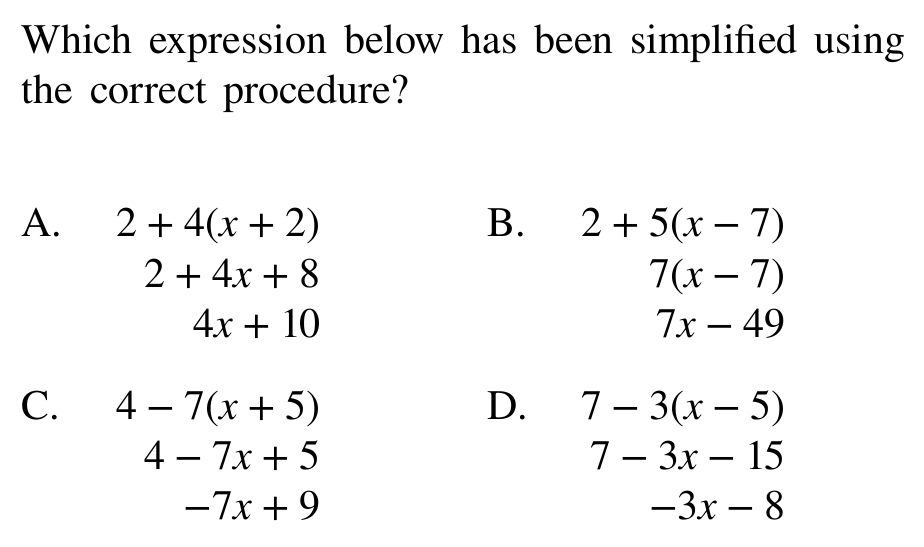
\includegraphics[width=0.8\linewidth]{SimplifyProcedure1}

\leavevmode\\\relax 



\medskip
\goodbreak
\hrule
\nobreak
\smallskip

    \ifx\pgmlMarker\undefined
      \newdimen\pgmlMarker \pgmlMarker=0.00314159pt  % hack to tell if \newline was used
    \fi
    \ifx\oldnewline\undefined \let\oldnewline=\newline \fi
    \def\newline{\oldnewline\hskip-\pgmlMarker\hskip\pgmlMarker\relax}%
    \parindent=0pt
    \catcode`\^^M=\active
    \def^^M{\ifmmode\else\fi\ignorespaces}%  skip paragraph breaks in the preamble
    \def\par{\ifmmode\else\endgraf\fi\ignorespaces}%
  
%%% BEGIN PROBLEM PREAMBLE
{\bf 12.} (1 point) \ifdim\lastskip=\pgmlMarker
  \let\pgmlPar=\relax
 \else
  \let\pgmlPar=\par
  \vadjust{\kern3pt}%
\fi

%%%%%%%%%%%%%%%%%%%%%%%%%%%%%%%%%%%%%%
%
%    definitions for PGML
%

\ifx\pgmlCount\undefined  % do not redefine if multiple files load PGML.pl
  \newcount\pgmlCount
  \newdimen\pgmlPercent
  \newdimen\pgmlPixels  \pgmlPixels=.5pt
\fi
\pgmlPercent=.01\hsize

\def\pgmlSetup{%
  \parskip=0pt \parindent=0pt
%  \ifdim\lastskip=\pgmlMarker\else\par\fi
  \pgmlPar
}%

\def\pgmlIndent{\par\advance\leftskip by 2em \advance\pgmlPercent by .02em \pgmlCount=0}%
\def\pgmlbulletItem{\par\indent\llap{$\bullet$ }\ignorespaces}%
\def\pgmlcircleItem{\par\indent\llap{$\circ$ }\ignorespaces}%
\def\pgmlsquareItem{\par\indent\llap{\vrule height 1ex width .75ex depth -.25ex\ }\ignorespaces}%
\def\pgmlnumericItem{\par\indent\advance\pgmlCount by 1 \llap{\the\pgmlCount. }\ignorespaces}%
\def\pgmlalphaItem{\par\indent{\advance\pgmlCount by `\a \llap{\char\pgmlCount. }}\advance\pgmlCount by 1\ignorespaces}%
\def\pgmlAlphaItem{\par\indent{\advance\pgmlCount by `\A \llap{\char\pgmlCount. }}\advance\pgmlCount by 1\ignorespaces}%
\def\pgmlromanItem{\par\indent\advance\pgmlCount by 1 \llap{\romannumeral\pgmlCount. }\ignorespaces}%
\def\pgmlRomanItem{\par\indent\advance\pgmlCount by 1 \llap{\uppercase\expandafter{\romannumeral\pgmlCount}. }\ignorespaces}%

\def\pgmlCenter{%
  \par \parfillskip=0pt
  \advance\leftskip by 0pt plus .5\hsize
  \advance\rightskip by 0pt plus .5\hsize
  \def\pgmlBreak{\break}%
}%
\def\pgmlRight{%
  \par \parfillskip=0pt
  \advance\leftskip by 0pt plus \hsize
  \def\pgmlBreak{\break}%
}%

\def\pgmlBreak{\\}%

\def\pgmlHeading#1{%
  \par\bfseries
  \ifcase#1 \or\huge \or\LARGE \or\large \or\normalsize \or\footnotesize \or\scriptsize \fi
}%

\def\pgmlRule#1#2{%
  \par\noindent
  \hbox{%
    \strut%
    \dimen1=\ht\strutbox%
    \advance\dimen1 by -#2%
    \divide\dimen1 by 2%
    \advance\dimen2 by -\dp\strutbox%
    \raise\dimen1\hbox{\vrule width #1 height #2 depth 0pt}%
  }%
  \par
}%

\def\pgmlIC#1{\futurelet\pgmlNext\pgmlCheckIC}%
\def\pgmlCheckIC{\ifx\pgmlNext\pgmlSpace \/\fi}%
{\def\getSpace#1{\global\let\pgmlSpace= }\getSpace{} }%

{\catcode`\ =12\global\let\pgmlSpaceChar= }%
{\obeylines\gdef\pgmlPreformatted{\par\small\ttfamily\hsize=10\hsize\obeyspaces\obeylines\let^^M=\pgmlNL\pgmlNL}}%
\def\pgmlNL{\par\bgroup\catcode`\ =12\pgmlTestSpace}%
\def\pgmlTestSpace{\futurelet\next\pgmlTestChar}%
\def\pgmlTestChar{\ifx\next\pgmlSpaceChar\ \pgmlTestNext\fi\egroup}%
\def\pgmlTestNext\fi\egroup#1{\fi\pgmlTestSpace}%

\def^^M{\ifmmode\else\space\fi\ignorespaces}%
%%%%%%%%%%%%%%%%%%%%%%%%%%%%%%%%%%%%%%

%%% END PROBLEM PREAMBLE
The table below shows how many scoops of
hot chocolate mix are needed in order to make
di erent numbers of cups of hot chocolate.

\par 
\par\begin{minipage}{\linewidth}\centering\captionsetup{textfont={sc},belowskip=12pt,aboveskip=4pt}\captionof*{table}{Hot Chocolate Mix Recipe}\begin{tabular}{l | c | c | c | c}\toprule \bfseries  Number of cups of Hot Chocolate (c) &  2 &  4 &  6 &  8 \\\midrule  \bfseries  Number of scoops of Mix Needed (s) &  4 &  8 &  12 &  16 \\\bottomrule\end{tabular}\end{minipage}\par  \vspace{1pc}


Write an equation that can be used to find the number of scoops (s) of hot chocolate mix needed to make c cups of hot chocolate.

\vspace{0.25cm}\\
\mbox{\parbox[t]{25ex}{\hrulefill}}



\medskip
\goodbreak
\hrule
\nobreak
\smallskip

%%% BEGIN PROBLEM PREAMBLE
{\bf 13.} (1 point) \ifdim\lastskip=\pgmlMarker
  \let\pgmlPar=\relax
 \else
  \let\pgmlPar=\par
  \vadjust{\kern3pt}%
\fi

%%%%%%%%%%%%%%%%%%%%%%%%%%%%%%%%%%%%%%
%
%    definitions for PGML
%

\ifx\pgmlCount\undefined  % do not redefine if multiple files load PGML.pl
  \newcount\pgmlCount
  \newdimen\pgmlPercent
  \newdimen\pgmlPixels  \pgmlPixels=.5pt
\fi
\pgmlPercent=.01\hsize

\def\pgmlSetup{%
  \parskip=0pt \parindent=0pt
%  \ifdim\lastskip=\pgmlMarker\else\par\fi
  \pgmlPar
}%

\def\pgmlIndent{\par\advance\leftskip by 2em \advance\pgmlPercent by .02em \pgmlCount=0}%
\def\pgmlbulletItem{\par\indent\llap{$\bullet$ }\ignorespaces}%
\def\pgmlcircleItem{\par\indent\llap{$\circ$ }\ignorespaces}%
\def\pgmlsquareItem{\par\indent\llap{\vrule height 1ex width .75ex depth -.25ex\ }\ignorespaces}%
\def\pgmlnumericItem{\par\indent\advance\pgmlCount by 1 \llap{\the\pgmlCount. }\ignorespaces}%
\def\pgmlalphaItem{\par\indent{\advance\pgmlCount by `\a \llap{\char\pgmlCount. }}\advance\pgmlCount by 1\ignorespaces}%
\def\pgmlAlphaItem{\par\indent{\advance\pgmlCount by `\A \llap{\char\pgmlCount. }}\advance\pgmlCount by 1\ignorespaces}%
\def\pgmlromanItem{\par\indent\advance\pgmlCount by 1 \llap{\romannumeral\pgmlCount. }\ignorespaces}%
\def\pgmlRomanItem{\par\indent\advance\pgmlCount by 1 \llap{\uppercase\expandafter{\romannumeral\pgmlCount}. }\ignorespaces}%

\def\pgmlCenter{%
  \par \parfillskip=0pt
  \advance\leftskip by 0pt plus .5\hsize
  \advance\rightskip by 0pt plus .5\hsize
  \def\pgmlBreak{\break}%
}%
\def\pgmlRight{%
  \par \parfillskip=0pt
  \advance\leftskip by 0pt plus \hsize
  \def\pgmlBreak{\break}%
}%

\def\pgmlBreak{\\}%

\def\pgmlHeading#1{%
  \par\bfseries
  \ifcase#1 \or\huge \or\LARGE \or\large \or\normalsize \or\footnotesize \or\scriptsize \fi
}%

\def\pgmlRule#1#2{%
  \par\noindent
  \hbox{%
    \strut%
    \dimen1=\ht\strutbox%
    \advance\dimen1 by -#2%
    \divide\dimen1 by 2%
    \advance\dimen2 by -\dp\strutbox%
    \raise\dimen1\hbox{\vrule width #1 height #2 depth 0pt}%
  }%
  \par
}%

\def\pgmlIC#1{\futurelet\pgmlNext\pgmlCheckIC}%
\def\pgmlCheckIC{\ifx\pgmlNext\pgmlSpace \/\fi}%
{\def\getSpace#1{\global\let\pgmlSpace= }\getSpace{} }%

{\catcode`\ =12\global\let\pgmlSpaceChar= }%
{\obeylines\gdef\pgmlPreformatted{\par\small\ttfamily\hsize=10\hsize\obeyspaces\obeylines\let^^M=\pgmlNL\pgmlNL}}%
\def\pgmlNL{\par\bgroup\catcode`\ =12\pgmlTestSpace}%
\def\pgmlTestSpace{\futurelet\next\pgmlTestChar}%
\def\pgmlTestChar{\ifx\next\pgmlSpaceChar\ \pgmlTestNext\fi\egroup}%
\def\pgmlTestNext\fi\egroup#1{\fi\pgmlTestSpace}%

\def^^M{\ifmmode\else\space\fi\ignorespaces}%
%%%%%%%%%%%%%%%%%%%%%%%%%%%%%%%%%%%%%%

%%% END PROBLEM PREAMBLE
What expression is the result when \(2a - 5\)
subtracted from \(3a + 3\) ? Put your answer in simplest (standard) form.

\vspace{0.25cm}
\par 
\mbox{\parbox[t]{25ex}{\hrulefill}}



\medskip
\goodbreak
\hrule
\nobreak
\smallskip

    \ifx\pgmlMarker\undefined
      \newdimen\pgmlMarker \pgmlMarker=0.00314159pt  % hack to tell if \newline was used
    \fi
    \ifx\oldnewline\undefined \let\oldnewline=\newline \fi
    \def\newline{\oldnewline\hskip-\pgmlMarker\hskip\pgmlMarker\relax}%
    \parindent=0pt
    \catcode`\^^M=\active
    \def^^M{\ifmmode\else\fi\ignorespaces}%  skip paragraph breaks in the preamble
    \def\par{\ifmmode\else\endgraf\fi\ignorespaces}%
  
%%% BEGIN PROBLEM PREAMBLE
{\bf 14.} (1 point) \ifdim\lastskip=\pgmlMarker
  \let\pgmlPar=\relax
 \else
  \let\pgmlPar=\par
  \vadjust{\kern3pt}%
\fi

%%%%%%%%%%%%%%%%%%%%%%%%%%%%%%%%%%%%%%
%
%    definitions for PGML
%

\ifx\pgmlCount\undefined  % do not redefine if multiple files load PGML.pl
  \newcount\pgmlCount
  \newdimen\pgmlPercent
  \newdimen\pgmlPixels  \pgmlPixels=.5pt
\fi
\pgmlPercent=.01\hsize

\def\pgmlSetup{%
  \parskip=0pt \parindent=0pt
%  \ifdim\lastskip=\pgmlMarker\else\par\fi
  \pgmlPar
}%

\def\pgmlIndent{\par\advance\leftskip by 2em \advance\pgmlPercent by .02em \pgmlCount=0}%
\def\pgmlbulletItem{\par\indent\llap{$\bullet$ }\ignorespaces}%
\def\pgmlcircleItem{\par\indent\llap{$\circ$ }\ignorespaces}%
\def\pgmlsquareItem{\par\indent\llap{\vrule height 1ex width .75ex depth -.25ex\ }\ignorespaces}%
\def\pgmlnumericItem{\par\indent\advance\pgmlCount by 1 \llap{\the\pgmlCount. }\ignorespaces}%
\def\pgmlalphaItem{\par\indent{\advance\pgmlCount by `\a \llap{\char\pgmlCount. }}\advance\pgmlCount by 1\ignorespaces}%
\def\pgmlAlphaItem{\par\indent{\advance\pgmlCount by `\A \llap{\char\pgmlCount. }}\advance\pgmlCount by 1\ignorespaces}%
\def\pgmlromanItem{\par\indent\advance\pgmlCount by 1 \llap{\romannumeral\pgmlCount. }\ignorespaces}%
\def\pgmlRomanItem{\par\indent\advance\pgmlCount by 1 \llap{\uppercase\expandafter{\romannumeral\pgmlCount}. }\ignorespaces}%

\def\pgmlCenter{%
  \par \parfillskip=0pt
  \advance\leftskip by 0pt plus .5\hsize
  \advance\rightskip by 0pt plus .5\hsize
  \def\pgmlBreak{\break}%
}%
\def\pgmlRight{%
  \par \parfillskip=0pt
  \advance\leftskip by 0pt plus \hsize
  \def\pgmlBreak{\break}%
}%

\def\pgmlBreak{\\}%

\def\pgmlHeading#1{%
  \par\bfseries
  \ifcase#1 \or\huge \or\LARGE \or\large \or\normalsize \or\footnotesize \or\scriptsize \fi
}%

\def\pgmlRule#1#2{%
  \par\noindent
  \hbox{%
    \strut%
    \dimen1=\ht\strutbox%
    \advance\dimen1 by -#2%
    \divide\dimen1 by 2%
    \advance\dimen2 by -\dp\strutbox%
    \raise\dimen1\hbox{\vrule width #1 height #2 depth 0pt}%
  }%
  \par
}%

\def\pgmlIC#1{\futurelet\pgmlNext\pgmlCheckIC}%
\def\pgmlCheckIC{\ifx\pgmlNext\pgmlSpace \/\fi}%
{\def\getSpace#1{\global\let\pgmlSpace= }\getSpace{} }%

{\catcode`\ =12\global\let\pgmlSpaceChar= }%
{\obeylines\gdef\pgmlPreformatted{\par\small\ttfamily\hsize=10\hsize\obeyspaces\obeylines\let^^M=\pgmlNL\pgmlNL}}%
\def\pgmlNL{\par\bgroup\catcode`\ =12\pgmlTestSpace}%
\def\pgmlTestSpace{\futurelet\next\pgmlTestChar}%
\def\pgmlTestChar{\ifx\next\pgmlSpaceChar\ \pgmlTestNext\fi\egroup}%
\def\pgmlTestNext\fi\egroup#1{\fi\pgmlTestSpace}%

\def^^M{\ifmmode\else\space\fi\ignorespaces}%
%%%%%%%%%%%%%%%%%%%%%%%%%%%%%%%%%%%%%%

%%% END PROBLEM PREAMBLE

\leavevmode\\\relax 
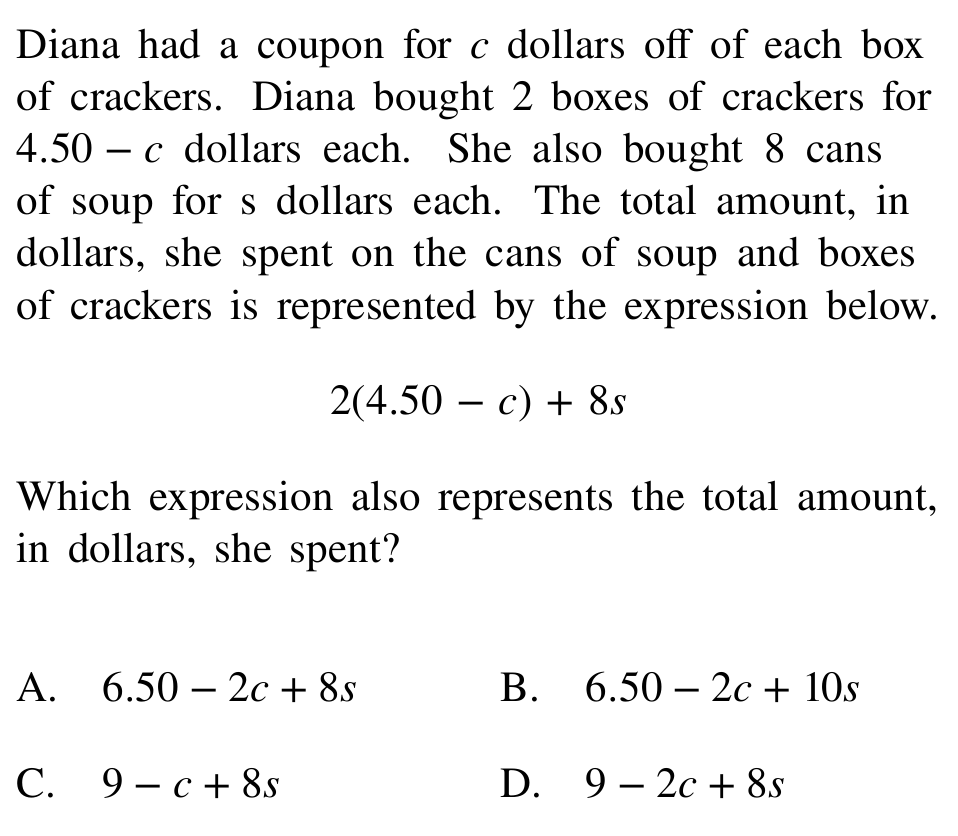
\includegraphics[width=0.8\linewidth]{EquivalentExpressionInContext1}

\leavevmode\\\relax 



\medskip
\goodbreak
\hrule
\nobreak
\smallskip

    \ifx\pgmlMarker\undefined
      \newdimen\pgmlMarker \pgmlMarker=0.00314159pt  % hack to tell if \newline was used
    \fi
    \ifx\oldnewline\undefined \let\oldnewline=\newline \fi
    \def\newline{\oldnewline\hskip-\pgmlMarker\hskip\pgmlMarker\relax}%
    \parindent=0pt
    \catcode`\^^M=\active
    \def^^M{\ifmmode\else\fi\ignorespaces}%  skip paragraph breaks in the preamble
    \def\par{\ifmmode\else\endgraf\fi\ignorespaces}%
  
%%% BEGIN PROBLEM PREAMBLE
{\bf 15.} (1 point) \ifdim\lastskip=\pgmlMarker
  \let\pgmlPar=\relax
 \else
  \let\pgmlPar=\par
  \vadjust{\kern3pt}%
\fi

%%%%%%%%%%%%%%%%%%%%%%%%%%%%%%%%%%%%%%
%
%    definitions for PGML
%

\ifx\pgmlCount\undefined  % do not redefine if multiple files load PGML.pl
  \newcount\pgmlCount
  \newdimen\pgmlPercent
  \newdimen\pgmlPixels  \pgmlPixels=.5pt
\fi
\pgmlPercent=.01\hsize

\def\pgmlSetup{%
  \parskip=0pt \parindent=0pt
%  \ifdim\lastskip=\pgmlMarker\else\par\fi
  \pgmlPar
}%

\def\pgmlIndent{\par\advance\leftskip by 2em \advance\pgmlPercent by .02em \pgmlCount=0}%
\def\pgmlbulletItem{\par\indent\llap{$\bullet$ }\ignorespaces}%
\def\pgmlcircleItem{\par\indent\llap{$\circ$ }\ignorespaces}%
\def\pgmlsquareItem{\par\indent\llap{\vrule height 1ex width .75ex depth -.25ex\ }\ignorespaces}%
\def\pgmlnumericItem{\par\indent\advance\pgmlCount by 1 \llap{\the\pgmlCount. }\ignorespaces}%
\def\pgmlalphaItem{\par\indent{\advance\pgmlCount by `\a \llap{\char\pgmlCount. }}\advance\pgmlCount by 1\ignorespaces}%
\def\pgmlAlphaItem{\par\indent{\advance\pgmlCount by `\A \llap{\char\pgmlCount. }}\advance\pgmlCount by 1\ignorespaces}%
\def\pgmlromanItem{\par\indent\advance\pgmlCount by 1 \llap{\romannumeral\pgmlCount. }\ignorespaces}%
\def\pgmlRomanItem{\par\indent\advance\pgmlCount by 1 \llap{\uppercase\expandafter{\romannumeral\pgmlCount}. }\ignorespaces}%

\def\pgmlCenter{%
  \par \parfillskip=0pt
  \advance\leftskip by 0pt plus .5\hsize
  \advance\rightskip by 0pt plus .5\hsize
  \def\pgmlBreak{\break}%
}%
\def\pgmlRight{%
  \par \parfillskip=0pt
  \advance\leftskip by 0pt plus \hsize
  \def\pgmlBreak{\break}%
}%

\def\pgmlBreak{\\}%

\def\pgmlHeading#1{%
  \par\bfseries
  \ifcase#1 \or\huge \or\LARGE \or\large \or\normalsize \or\footnotesize \or\scriptsize \fi
}%

\def\pgmlRule#1#2{%
  \par\noindent
  \hbox{%
    \strut%
    \dimen1=\ht\strutbox%
    \advance\dimen1 by -#2%
    \divide\dimen1 by 2%
    \advance\dimen2 by -\dp\strutbox%
    \raise\dimen1\hbox{\vrule width #1 height #2 depth 0pt}%
  }%
  \par
}%

\def\pgmlIC#1{\futurelet\pgmlNext\pgmlCheckIC}%
\def\pgmlCheckIC{\ifx\pgmlNext\pgmlSpace \/\fi}%
{\def\getSpace#1{\global\let\pgmlSpace= }\getSpace{} }%

{\catcode`\ =12\global\let\pgmlSpaceChar= }%
{\obeylines\gdef\pgmlPreformatted{\par\small\ttfamily\hsize=10\hsize\obeyspaces\obeylines\let^^M=\pgmlNL\pgmlNL}}%
\def\pgmlNL{\par\bgroup\catcode`\ =12\pgmlTestSpace}%
\def\pgmlTestSpace{\futurelet\next\pgmlTestChar}%
\def\pgmlTestChar{\ifx\next\pgmlSpaceChar\ \pgmlTestNext\fi\egroup}%
\def\pgmlTestNext\fi\egroup#1{\fi\pgmlTestSpace}%

\def^^M{\ifmmode\else\space\fi\ignorespaces}%
%%%%%%%%%%%%%%%%%%%%%%%%%%%%%%%%%%%%%%

%%% END PROBLEM PREAMBLE

A. Leo bought a used car for \(x\) dollars. One year
later, the value of the car was \(0.88x\). Which
expression is another way to describe the change
in the value of the car?

\leavevmode\\\relax 

\par\vtop{\def\bitem{\hbox\bgroup\indent\strut\textbullet\ \ignorespaces}\let\eitem=\egroup
\bitem \verb�0.12% decrease�\eitem
\bitem \verb�0.88% decrease�\eitem
\bitem \verb�12% decrease�\eitem
\bitem \verb�88% decrease�\eitem
\vskip3pt}


\leavevmode\\\relax 
B. Based on the answer to A, Leo wrote the following expression to represent the new value of the car. 

\leavevmode\\\relax 
\begin{center}
\(x - 0.12 x\)
\end{center}

\leavevmode\\\relax 
For parts B and C, use the particular value \(x=3500\) to test whether the two expressions are equivalent.

\leavevmode\\\relax 
B. What is the value of the expression \(0.88 x\) if  \(x = 3500\)?

\vspace{0.25cm}\\
\mbox{\parbox[t]{25ex}{\hrulefill}}.

\leavevmode\\\relax 
C. What is the value of the expression \(x - 0.12 x\) if \(x = 3500\)?

\vspace{0.25cm}\\
\mbox{\parbox[t]{25ex}{\hrulefill}}.

\leavevmode\\\relax 
D. Is the expression \(x - 0.12 x\) equivalent to \(0.88 x\)?

\vspace{0.5cm}

\leavevmode\\\relax 
E. Justify your answer to part D.
\vskip 4 in \hrulefill\quad 



\medskip
\goodbreak
\hrule
\nobreak
\smallskip

    \ifx\pgmlMarker\undefined
      \newdimen\pgmlMarker \pgmlMarker=0.00314159pt  % hack to tell if \newline was used
    \fi
    \ifx\oldnewline\undefined \let\oldnewline=\newline \fi
    \def\newline{\oldnewline\hskip-\pgmlMarker\hskip\pgmlMarker\relax}%
    \parindent=0pt
    \catcode`\^^M=\active
    \def^^M{\ifmmode\else\fi\ignorespaces}%  skip paragraph breaks in the preamble
    \def\par{\ifmmode\else\endgraf\fi\ignorespaces}%
  
%%% BEGIN PROBLEM PREAMBLE
{\bf 16.} (1 point) \ifdim\lastskip=\pgmlMarker
  \let\pgmlPar=\relax
 \else
  \let\pgmlPar=\par
  \vadjust{\kern3pt}%
\fi

%%%%%%%%%%%%%%%%%%%%%%%%%%%%%%%%%%%%%%
%
%    definitions for PGML
%

\ifx\pgmlCount\undefined  % do not redefine if multiple files load PGML.pl
  \newcount\pgmlCount
  \newdimen\pgmlPercent
  \newdimen\pgmlPixels  \pgmlPixels=.5pt
\fi
\pgmlPercent=.01\hsize

\def\pgmlSetup{%
  \parskip=0pt \parindent=0pt
%  \ifdim\lastskip=\pgmlMarker\else\par\fi
  \pgmlPar
}%

\def\pgmlIndent{\par\advance\leftskip by 2em \advance\pgmlPercent by .02em \pgmlCount=0}%
\def\pgmlbulletItem{\par\indent\llap{$\bullet$ }\ignorespaces}%
\def\pgmlcircleItem{\par\indent\llap{$\circ$ }\ignorespaces}%
\def\pgmlsquareItem{\par\indent\llap{\vrule height 1ex width .75ex depth -.25ex\ }\ignorespaces}%
\def\pgmlnumericItem{\par\indent\advance\pgmlCount by 1 \llap{\the\pgmlCount. }\ignorespaces}%
\def\pgmlalphaItem{\par\indent{\advance\pgmlCount by `\a \llap{\char\pgmlCount. }}\advance\pgmlCount by 1\ignorespaces}%
\def\pgmlAlphaItem{\par\indent{\advance\pgmlCount by `\A \llap{\char\pgmlCount. }}\advance\pgmlCount by 1\ignorespaces}%
\def\pgmlromanItem{\par\indent\advance\pgmlCount by 1 \llap{\romannumeral\pgmlCount. }\ignorespaces}%
\def\pgmlRomanItem{\par\indent\advance\pgmlCount by 1 \llap{\uppercase\expandafter{\romannumeral\pgmlCount}. }\ignorespaces}%

\def\pgmlCenter{%
  \par \parfillskip=0pt
  \advance\leftskip by 0pt plus .5\hsize
  \advance\rightskip by 0pt plus .5\hsize
  \def\pgmlBreak{\break}%
}%
\def\pgmlRight{%
  \par \parfillskip=0pt
  \advance\leftskip by 0pt plus \hsize
  \def\pgmlBreak{\break}%
}%

\def\pgmlBreak{\\}%

\def\pgmlHeading#1{%
  \par\bfseries
  \ifcase#1 \or\huge \or\LARGE \or\large \or\normalsize \or\footnotesize \or\scriptsize \fi
}%

\def\pgmlRule#1#2{%
  \par\noindent
  \hbox{%
    \strut%
    \dimen1=\ht\strutbox%
    \advance\dimen1 by -#2%
    \divide\dimen1 by 2%
    \advance\dimen2 by -\dp\strutbox%
    \raise\dimen1\hbox{\vrule width #1 height #2 depth 0pt}%
  }%
  \par
}%

\def\pgmlIC#1{\futurelet\pgmlNext\pgmlCheckIC}%
\def\pgmlCheckIC{\ifx\pgmlNext\pgmlSpace \/\fi}%
{\def\getSpace#1{\global\let\pgmlSpace= }\getSpace{} }%

{\catcode`\ =12\global\let\pgmlSpaceChar= }%
{\obeylines\gdef\pgmlPreformatted{\par\small\ttfamily\hsize=10\hsize\obeyspaces\obeylines\let^^M=\pgmlNL\pgmlNL}}%
\def\pgmlNL{\par\bgroup\catcode`\ =12\pgmlTestSpace}%
\def\pgmlTestSpace{\futurelet\next\pgmlTestChar}%
\def\pgmlTestChar{\ifx\next\pgmlSpaceChar\ \pgmlTestNext\fi\egroup}%
\def\pgmlTestNext\fi\egroup#1{\fi\pgmlTestSpace}%

\def^^M{\ifmmode\else\space\fi\ignorespaces}%
%%%%%%%%%%%%%%%%%%%%%%%%%%%%%%%%%%%%%%

%%% END PROBLEM PREAMBLE
{\pgmlSetup
Use the distributive property to write an equivalent expression that has no grouping symbols.
\vskip\baselineskip
{\pgmlIndent
\({-\left(B+6\right)}\)
\vskip\baselineskip
\(=\) \mbox{\parbox[t]{7ex}{\hrulefill}} 
\par}%
\vskip\baselineskip
\par}%

\medskip
\goodbreak
\hrule
\nobreak
\smallskip

%%% BEGIN PROBLEM PREAMBLE
{\bf 17.} (1 point) \ifdim\lastskip=\pgmlMarker
  \let\pgmlPar=\relax
 \else
  \let\pgmlPar=\par
  \vadjust{\kern3pt}%
\fi

%%%%%%%%%%%%%%%%%%%%%%%%%%%%%%%%%%%%%%
%
%    definitions for PGML
%

\ifx\pgmlCount\undefined  % do not redefine if multiple files load PGML.pl
  \newcount\pgmlCount
  \newdimen\pgmlPercent
  \newdimen\pgmlPixels  \pgmlPixels=.5pt
\fi
\pgmlPercent=.01\hsize

\def\pgmlSetup{%
  \parskip=0pt \parindent=0pt
%  \ifdim\lastskip=\pgmlMarker\else\par\fi
  \pgmlPar
}%

\def\pgmlIndent{\par\advance\leftskip by 2em \advance\pgmlPercent by .02em \pgmlCount=0}%
\def\pgmlbulletItem{\par\indent\llap{$\bullet$ }\ignorespaces}%
\def\pgmlcircleItem{\par\indent\llap{$\circ$ }\ignorespaces}%
\def\pgmlsquareItem{\par\indent\llap{\vrule height 1ex width .75ex depth -.25ex\ }\ignorespaces}%
\def\pgmlnumericItem{\par\indent\advance\pgmlCount by 1 \llap{\the\pgmlCount. }\ignorespaces}%
\def\pgmlalphaItem{\par\indent{\advance\pgmlCount by `\a \llap{\char\pgmlCount. }}\advance\pgmlCount by 1\ignorespaces}%
\def\pgmlAlphaItem{\par\indent{\advance\pgmlCount by `\A \llap{\char\pgmlCount. }}\advance\pgmlCount by 1\ignorespaces}%
\def\pgmlromanItem{\par\indent\advance\pgmlCount by 1 \llap{\romannumeral\pgmlCount. }\ignorespaces}%
\def\pgmlRomanItem{\par\indent\advance\pgmlCount by 1 \llap{\uppercase\expandafter{\romannumeral\pgmlCount}. }\ignorespaces}%

\def\pgmlCenter{%
  \par \parfillskip=0pt
  \advance\leftskip by 0pt plus .5\hsize
  \advance\rightskip by 0pt plus .5\hsize
  \def\pgmlBreak{\break}%
}%
\def\pgmlRight{%
  \par \parfillskip=0pt
  \advance\leftskip by 0pt plus \hsize
  \def\pgmlBreak{\break}%
}%

\def\pgmlBreak{\\}%

\def\pgmlHeading#1{%
  \par\bfseries
  \ifcase#1 \or\huge \or\LARGE \or\large \or\normalsize \or\footnotesize \or\scriptsize \fi
}%

\def\pgmlRule#1#2{%
  \par\noindent
  \hbox{%
    \strut%
    \dimen1=\ht\strutbox%
    \advance\dimen1 by -#2%
    \divide\dimen1 by 2%
    \advance\dimen2 by -\dp\strutbox%
    \raise\dimen1\hbox{\vrule width #1 height #2 depth 0pt}%
  }%
  \par
}%

\def\pgmlIC#1{\futurelet\pgmlNext\pgmlCheckIC}%
\def\pgmlCheckIC{\ifx\pgmlNext\pgmlSpace \/\fi}%
{\def\getSpace#1{\global\let\pgmlSpace= }\getSpace{} }%

{\catcode`\ =12\global\let\pgmlSpaceChar= }%
{\obeylines\gdef\pgmlPreformatted{\par\small\ttfamily\hsize=10\hsize\obeyspaces\obeylines\let^^M=\pgmlNL\pgmlNL}}%
\def\pgmlNL{\par\bgroup\catcode`\ =12\pgmlTestSpace}%
\def\pgmlTestSpace{\futurelet\next\pgmlTestChar}%
\def\pgmlTestChar{\ifx\next\pgmlSpaceChar\ \pgmlTestNext\fi\egroup}%
\def\pgmlTestNext\fi\egroup#1{\fi\pgmlTestSpace}%

\def^^M{\ifmmode\else\space\fi\ignorespaces}%
%%%%%%%%%%%%%%%%%%%%%%%%%%%%%%%%%%%%%%

%%% END PROBLEM PREAMBLE

Write each of these as a sum of two terms using the distributive law.
\vspace{0.25cm}
\par 
\(5(x+5)\)= \mbox{\parbox[t]{25ex}{\hrulefill}}
\par 



\medskip
\goodbreak
\hrule
\nobreak
\smallskip

%%% BEGIN PROBLEM PREAMBLE
{\bf 18.} (1 point) \ifdim\lastskip=\pgmlMarker
  \let\pgmlPar=\relax
 \else
  \let\pgmlPar=\par
  \vadjust{\kern3pt}%
\fi

%%%%%%%%%%%%%%%%%%%%%%%%%%%%%%%%%%%%%%
%
%    definitions for PGML
%

\ifx\pgmlCount\undefined  % do not redefine if multiple files load PGML.pl
  \newcount\pgmlCount
  \newdimen\pgmlPercent
  \newdimen\pgmlPixels  \pgmlPixels=.5pt
\fi
\pgmlPercent=.01\hsize

\def\pgmlSetup{%
  \parskip=0pt \parindent=0pt
%  \ifdim\lastskip=\pgmlMarker\else\par\fi
  \pgmlPar
}%

\def\pgmlIndent{\par\advance\leftskip by 2em \advance\pgmlPercent by .02em \pgmlCount=0}%
\def\pgmlbulletItem{\par\indent\llap{$\bullet$ }\ignorespaces}%
\def\pgmlcircleItem{\par\indent\llap{$\circ$ }\ignorespaces}%
\def\pgmlsquareItem{\par\indent\llap{\vrule height 1ex width .75ex depth -.25ex\ }\ignorespaces}%
\def\pgmlnumericItem{\par\indent\advance\pgmlCount by 1 \llap{\the\pgmlCount. }\ignorespaces}%
\def\pgmlalphaItem{\par\indent{\advance\pgmlCount by `\a \llap{\char\pgmlCount. }}\advance\pgmlCount by 1\ignorespaces}%
\def\pgmlAlphaItem{\par\indent{\advance\pgmlCount by `\A \llap{\char\pgmlCount. }}\advance\pgmlCount by 1\ignorespaces}%
\def\pgmlromanItem{\par\indent\advance\pgmlCount by 1 \llap{\romannumeral\pgmlCount. }\ignorespaces}%
\def\pgmlRomanItem{\par\indent\advance\pgmlCount by 1 \llap{\uppercase\expandafter{\romannumeral\pgmlCount}. }\ignorespaces}%

\def\pgmlCenter{%
  \par \parfillskip=0pt
  \advance\leftskip by 0pt plus .5\hsize
  \advance\rightskip by 0pt plus .5\hsize
  \def\pgmlBreak{\break}%
}%
\def\pgmlRight{%
  \par \parfillskip=0pt
  \advance\leftskip by 0pt plus \hsize
  \def\pgmlBreak{\break}%
}%

\def\pgmlBreak{\\}%

\def\pgmlHeading#1{%
  \par\bfseries
  \ifcase#1 \or\huge \or\LARGE \or\large \or\normalsize \or\footnotesize \or\scriptsize \fi
}%

\def\pgmlRule#1#2{%
  \par\noindent
  \hbox{%
    \strut%
    \dimen1=\ht\strutbox%
    \advance\dimen1 by -#2%
    \divide\dimen1 by 2%
    \advance\dimen2 by -\dp\strutbox%
    \raise\dimen1\hbox{\vrule width #1 height #2 depth 0pt}%
  }%
  \par
}%

\def\pgmlIC#1{\futurelet\pgmlNext\pgmlCheckIC}%
\def\pgmlCheckIC{\ifx\pgmlNext\pgmlSpace \/\fi}%
{\def\getSpace#1{\global\let\pgmlSpace= }\getSpace{} }%

{\catcode`\ =12\global\let\pgmlSpaceChar= }%
{\obeylines\gdef\pgmlPreformatted{\par\small\ttfamily\hsize=10\hsize\obeyspaces\obeylines\let^^M=\pgmlNL\pgmlNL}}%
\def\pgmlNL{\par\bgroup\catcode`\ =12\pgmlTestSpace}%
\def\pgmlTestSpace{\futurelet\next\pgmlTestChar}%
\def\pgmlTestChar{\ifx\next\pgmlSpaceChar\ \pgmlTestNext\fi\egroup}%
\def\pgmlTestNext\fi\egroup#1{\fi\pgmlTestSpace}%

\def^^M{\ifmmode\else\space\fi\ignorespaces}%
%%%%%%%%%%%%%%%%%%%%%%%%%%%%%%%%%%%%%%

%%% END PROBLEM PREAMBLE
Write each of these as a sum of two terms using the distributive law.
\vspace{0.25cm}
\par 
\(-2(x+9)\)= \mbox{\parbox[t]{25ex}{\hrulefill}}
\par 



\medskip
\goodbreak
\hrule
\nobreak
\smallskip

%%% BEGIN PROBLEM PREAMBLE
{\bf 19.} (1 point) \ifdim\lastskip=\pgmlMarker
  \let\pgmlPar=\relax
 \else
  \let\pgmlPar=\par
  \vadjust{\kern3pt}%
\fi

%%%%%%%%%%%%%%%%%%%%%%%%%%%%%%%%%%%%%%
%
%    definitions for PGML
%

\ifx\pgmlCount\undefined  % do not redefine if multiple files load PGML.pl
  \newcount\pgmlCount
  \newdimen\pgmlPercent
  \newdimen\pgmlPixels  \pgmlPixels=.5pt
\fi
\pgmlPercent=.01\hsize

\def\pgmlSetup{%
  \parskip=0pt \parindent=0pt
%  \ifdim\lastskip=\pgmlMarker\else\par\fi
  \pgmlPar
}%

\def\pgmlIndent{\par\advance\leftskip by 2em \advance\pgmlPercent by .02em \pgmlCount=0}%
\def\pgmlbulletItem{\par\indent\llap{$\bullet$ }\ignorespaces}%
\def\pgmlcircleItem{\par\indent\llap{$\circ$ }\ignorespaces}%
\def\pgmlsquareItem{\par\indent\llap{\vrule height 1ex width .75ex depth -.25ex\ }\ignorespaces}%
\def\pgmlnumericItem{\par\indent\advance\pgmlCount by 1 \llap{\the\pgmlCount. }\ignorespaces}%
\def\pgmlalphaItem{\par\indent{\advance\pgmlCount by `\a \llap{\char\pgmlCount. }}\advance\pgmlCount by 1\ignorespaces}%
\def\pgmlAlphaItem{\par\indent{\advance\pgmlCount by `\A \llap{\char\pgmlCount. }}\advance\pgmlCount by 1\ignorespaces}%
\def\pgmlromanItem{\par\indent\advance\pgmlCount by 1 \llap{\romannumeral\pgmlCount. }\ignorespaces}%
\def\pgmlRomanItem{\par\indent\advance\pgmlCount by 1 \llap{\uppercase\expandafter{\romannumeral\pgmlCount}. }\ignorespaces}%

\def\pgmlCenter{%
  \par \parfillskip=0pt
  \advance\leftskip by 0pt plus .5\hsize
  \advance\rightskip by 0pt plus .5\hsize
  \def\pgmlBreak{\break}%
}%
\def\pgmlRight{%
  \par \parfillskip=0pt
  \advance\leftskip by 0pt plus \hsize
  \def\pgmlBreak{\break}%
}%

\def\pgmlBreak{\\}%

\def\pgmlHeading#1{%
  \par\bfseries
  \ifcase#1 \or\huge \or\LARGE \or\large \or\normalsize \or\footnotesize \or\scriptsize \fi
}%

\def\pgmlRule#1#2{%
  \par\noindent
  \hbox{%
    \strut%
    \dimen1=\ht\strutbox%
    \advance\dimen1 by -#2%
    \divide\dimen1 by 2%
    \advance\dimen2 by -\dp\strutbox%
    \raise\dimen1\hbox{\vrule width #1 height #2 depth 0pt}%
  }%
  \par
}%

\def\pgmlIC#1{\futurelet\pgmlNext\pgmlCheckIC}%
\def\pgmlCheckIC{\ifx\pgmlNext\pgmlSpace \/\fi}%
{\def\getSpace#1{\global\let\pgmlSpace= }\getSpace{} }%

{\catcode`\ =12\global\let\pgmlSpaceChar= }%
{\obeylines\gdef\pgmlPreformatted{\par\small\ttfamily\hsize=10\hsize\obeyspaces\obeylines\let^^M=\pgmlNL\pgmlNL}}%
\def\pgmlNL{\par\bgroup\catcode`\ =12\pgmlTestSpace}%
\def\pgmlTestSpace{\futurelet\next\pgmlTestChar}%
\def\pgmlTestChar{\ifx\next\pgmlSpaceChar\ \pgmlTestNext\fi\egroup}%
\def\pgmlTestNext\fi\egroup#1{\fi\pgmlTestSpace}%

\def^^M{\ifmmode\else\space\fi\ignorespaces}%
%%%%%%%%%%%%%%%%%%%%%%%%%%%%%%%%%%%%%%

%%% END PROBLEM PREAMBLE
Write each of these as a sum of two terms using the distributive law.
\vspace{0.25cm}
\par 
\(6(x-4)\)= \mbox{\parbox[t]{25ex}{\hrulefill}}
\par 



\medskip
\goodbreak
\hrule
\nobreak
\smallskip

%%% BEGIN PROBLEM PREAMBLE
{\bf 20.} (1 point) \ifdim\lastskip=\pgmlMarker
  \let\pgmlPar=\relax
 \else
  \let\pgmlPar=\par
  \vadjust{\kern3pt}%
\fi

%%%%%%%%%%%%%%%%%%%%%%%%%%%%%%%%%%%%%%
%
%    definitions for PGML
%

\ifx\pgmlCount\undefined  % do not redefine if multiple files load PGML.pl
  \newcount\pgmlCount
  \newdimen\pgmlPercent
  \newdimen\pgmlPixels  \pgmlPixels=.5pt
\fi
\pgmlPercent=.01\hsize

\def\pgmlSetup{%
  \parskip=0pt \parindent=0pt
%  \ifdim\lastskip=\pgmlMarker\else\par\fi
  \pgmlPar
}%

\def\pgmlIndent{\par\advance\leftskip by 2em \advance\pgmlPercent by .02em \pgmlCount=0}%
\def\pgmlbulletItem{\par\indent\llap{$\bullet$ }\ignorespaces}%
\def\pgmlcircleItem{\par\indent\llap{$\circ$ }\ignorespaces}%
\def\pgmlsquareItem{\par\indent\llap{\vrule height 1ex width .75ex depth -.25ex\ }\ignorespaces}%
\def\pgmlnumericItem{\par\indent\advance\pgmlCount by 1 \llap{\the\pgmlCount. }\ignorespaces}%
\def\pgmlalphaItem{\par\indent{\advance\pgmlCount by `\a \llap{\char\pgmlCount. }}\advance\pgmlCount by 1\ignorespaces}%
\def\pgmlAlphaItem{\par\indent{\advance\pgmlCount by `\A \llap{\char\pgmlCount. }}\advance\pgmlCount by 1\ignorespaces}%
\def\pgmlromanItem{\par\indent\advance\pgmlCount by 1 \llap{\romannumeral\pgmlCount. }\ignorespaces}%
\def\pgmlRomanItem{\par\indent\advance\pgmlCount by 1 \llap{\uppercase\expandafter{\romannumeral\pgmlCount}. }\ignorespaces}%

\def\pgmlCenter{%
  \par \parfillskip=0pt
  \advance\leftskip by 0pt plus .5\hsize
  \advance\rightskip by 0pt plus .5\hsize
  \def\pgmlBreak{\break}%
}%
\def\pgmlRight{%
  \par \parfillskip=0pt
  \advance\leftskip by 0pt plus \hsize
  \def\pgmlBreak{\break}%
}%

\def\pgmlBreak{\\}%

\def\pgmlHeading#1{%
  \par\bfseries
  \ifcase#1 \or\huge \or\LARGE \or\large \or\normalsize \or\footnotesize \or\scriptsize \fi
}%

\def\pgmlRule#1#2{%
  \par\noindent
  \hbox{%
    \strut%
    \dimen1=\ht\strutbox%
    \advance\dimen1 by -#2%
    \divide\dimen1 by 2%
    \advance\dimen2 by -\dp\strutbox%
    \raise\dimen1\hbox{\vrule width #1 height #2 depth 0pt}%
  }%
  \par
}%

\def\pgmlIC#1{\futurelet\pgmlNext\pgmlCheckIC}%
\def\pgmlCheckIC{\ifx\pgmlNext\pgmlSpace \/\fi}%
{\def\getSpace#1{\global\let\pgmlSpace= }\getSpace{} }%

{\catcode`\ =12\global\let\pgmlSpaceChar= }%
{\obeylines\gdef\pgmlPreformatted{\par\small\ttfamily\hsize=10\hsize\obeyspaces\obeylines\let^^M=\pgmlNL\pgmlNL}}%
\def\pgmlNL{\par\bgroup\catcode`\ =12\pgmlTestSpace}%
\def\pgmlTestSpace{\futurelet\next\pgmlTestChar}%
\def\pgmlTestChar{\ifx\next\pgmlSpaceChar\ \pgmlTestNext\fi\egroup}%
\def\pgmlTestNext\fi\egroup#1{\fi\pgmlTestSpace}%

\def^^M{\ifmmode\else\space\fi\ignorespaces}%
%%%%%%%%%%%%%%%%%%%%%%%%%%%%%%%%%%%%%%

%%% END PROBLEM PREAMBLE
Write each of these as a sum of two terms using the distributive law.
\vspace{0.25cm}
\par 
\(-3(x-3)\)= \mbox{\parbox[t]{25ex}{\hrulefill}}
\par 



\medskip
\goodbreak
\hrule
\nobreak
\smallskip

%%% BEGIN PROBLEM PREAMBLE
{\bf 21.} (1 point) \ifdim\lastskip=\pgmlMarker
  \let\pgmlPar=\relax
 \else
  \let\pgmlPar=\par
  \vadjust{\kern3pt}%
\fi

%%%%%%%%%%%%%%%%%%%%%%%%%%%%%%%%%%%%%%
%
%    definitions for PGML
%

\ifx\pgmlCount\undefined  % do not redefine if multiple files load PGML.pl
  \newcount\pgmlCount
  \newdimen\pgmlPercent
  \newdimen\pgmlPixels  \pgmlPixels=.5pt
\fi
\pgmlPercent=.01\hsize

\def\pgmlSetup{%
  \parskip=0pt \parindent=0pt
%  \ifdim\lastskip=\pgmlMarker\else\par\fi
  \pgmlPar
}%

\def\pgmlIndent{\par\advance\leftskip by 2em \advance\pgmlPercent by .02em \pgmlCount=0}%
\def\pgmlbulletItem{\par\indent\llap{$\bullet$ }\ignorespaces}%
\def\pgmlcircleItem{\par\indent\llap{$\circ$ }\ignorespaces}%
\def\pgmlsquareItem{\par\indent\llap{\vrule height 1ex width .75ex depth -.25ex\ }\ignorespaces}%
\def\pgmlnumericItem{\par\indent\advance\pgmlCount by 1 \llap{\the\pgmlCount. }\ignorespaces}%
\def\pgmlalphaItem{\par\indent{\advance\pgmlCount by `\a \llap{\char\pgmlCount. }}\advance\pgmlCount by 1\ignorespaces}%
\def\pgmlAlphaItem{\par\indent{\advance\pgmlCount by `\A \llap{\char\pgmlCount. }}\advance\pgmlCount by 1\ignorespaces}%
\def\pgmlromanItem{\par\indent\advance\pgmlCount by 1 \llap{\romannumeral\pgmlCount. }\ignorespaces}%
\def\pgmlRomanItem{\par\indent\advance\pgmlCount by 1 \llap{\uppercase\expandafter{\romannumeral\pgmlCount}. }\ignorespaces}%

\def\pgmlCenter{%
  \par \parfillskip=0pt
  \advance\leftskip by 0pt plus .5\hsize
  \advance\rightskip by 0pt plus .5\hsize
  \def\pgmlBreak{\break}%
}%
\def\pgmlRight{%
  \par \parfillskip=0pt
  \advance\leftskip by 0pt plus \hsize
  \def\pgmlBreak{\break}%
}%

\def\pgmlBreak{\\}%

\def\pgmlHeading#1{%
  \par\bfseries
  \ifcase#1 \or\huge \or\LARGE \or\large \or\normalsize \or\footnotesize \or\scriptsize \fi
}%

\def\pgmlRule#1#2{%
  \par\noindent
  \hbox{%
    \strut%
    \dimen1=\ht\strutbox%
    \advance\dimen1 by -#2%
    \divide\dimen1 by 2%
    \advance\dimen2 by -\dp\strutbox%
    \raise\dimen1\hbox{\vrule width #1 height #2 depth 0pt}%
  }%
  \par
}%

\def\pgmlIC#1{\futurelet\pgmlNext\pgmlCheckIC}%
\def\pgmlCheckIC{\ifx\pgmlNext\pgmlSpace \/\fi}%
{\def\getSpace#1{\global\let\pgmlSpace= }\getSpace{} }%

{\catcode`\ =12\global\let\pgmlSpaceChar= }%
{\obeylines\gdef\pgmlPreformatted{\par\small\ttfamily\hsize=10\hsize\obeyspaces\obeylines\let^^M=\pgmlNL\pgmlNL}}%
\def\pgmlNL{\par\bgroup\catcode`\ =12\pgmlTestSpace}%
\def\pgmlTestSpace{\futurelet\next\pgmlTestChar}%
\def\pgmlTestChar{\ifx\next\pgmlSpaceChar\ \pgmlTestNext\fi\egroup}%
\def\pgmlTestNext\fi\egroup#1{\fi\pgmlTestSpace}%

\def^^M{\ifmmode\else\space\fi\ignorespaces}%
%%%%%%%%%%%%%%%%%%%%%%%%%%%%%%%%%%%%%%

%%% END PROBLEM PREAMBLE
Write each of these as a sum of two terms using the distributive law.
\vspace{0.25cm}
\par 
\(3(4 x-9)\)= \mbox{\parbox[t]{25ex}{\hrulefill}}
\par 



\medskip
\goodbreak
\hrule
\nobreak
\smallskip

%%% BEGIN PROBLEM PREAMBLE
{\bf 22.} (1 point) \ifdim\lastskip=\pgmlMarker
  \let\pgmlPar=\relax
 \else
  \let\pgmlPar=\par
  \vadjust{\kern3pt}%
\fi

%%%%%%%%%%%%%%%%%%%%%%%%%%%%%%%%%%%%%%
%
%    definitions for PGML
%

\ifx\pgmlCount\undefined  % do not redefine if multiple files load PGML.pl
  \newcount\pgmlCount
  \newdimen\pgmlPercent
  \newdimen\pgmlPixels  \pgmlPixels=.5pt
\fi
\pgmlPercent=.01\hsize

\def\pgmlSetup{%
  \parskip=0pt \parindent=0pt
%  \ifdim\lastskip=\pgmlMarker\else\par\fi
  \pgmlPar
}%

\def\pgmlIndent{\par\advance\leftskip by 2em \advance\pgmlPercent by .02em \pgmlCount=0}%
\def\pgmlbulletItem{\par\indent\llap{$\bullet$ }\ignorespaces}%
\def\pgmlcircleItem{\par\indent\llap{$\circ$ }\ignorespaces}%
\def\pgmlsquareItem{\par\indent\llap{\vrule height 1ex width .75ex depth -.25ex\ }\ignorespaces}%
\def\pgmlnumericItem{\par\indent\advance\pgmlCount by 1 \llap{\the\pgmlCount. }\ignorespaces}%
\def\pgmlalphaItem{\par\indent{\advance\pgmlCount by `\a \llap{\char\pgmlCount. }}\advance\pgmlCount by 1\ignorespaces}%
\def\pgmlAlphaItem{\par\indent{\advance\pgmlCount by `\A \llap{\char\pgmlCount. }}\advance\pgmlCount by 1\ignorespaces}%
\def\pgmlromanItem{\par\indent\advance\pgmlCount by 1 \llap{\romannumeral\pgmlCount. }\ignorespaces}%
\def\pgmlRomanItem{\par\indent\advance\pgmlCount by 1 \llap{\uppercase\expandafter{\romannumeral\pgmlCount}. }\ignorespaces}%

\def\pgmlCenter{%
  \par \parfillskip=0pt
  \advance\leftskip by 0pt plus .5\hsize
  \advance\rightskip by 0pt plus .5\hsize
  \def\pgmlBreak{\break}%
}%
\def\pgmlRight{%
  \par \parfillskip=0pt
  \advance\leftskip by 0pt plus \hsize
  \def\pgmlBreak{\break}%
}%

\def\pgmlBreak{\\}%

\def\pgmlHeading#1{%
  \par\bfseries
  \ifcase#1 \or\huge \or\LARGE \or\large \or\normalsize \or\footnotesize \or\scriptsize \fi
}%

\def\pgmlRule#1#2{%
  \par\noindent
  \hbox{%
    \strut%
    \dimen1=\ht\strutbox%
    \advance\dimen1 by -#2%
    \divide\dimen1 by 2%
    \advance\dimen2 by -\dp\strutbox%
    \raise\dimen1\hbox{\vrule width #1 height #2 depth 0pt}%
  }%
  \par
}%

\def\pgmlIC#1{\futurelet\pgmlNext\pgmlCheckIC}%
\def\pgmlCheckIC{\ifx\pgmlNext\pgmlSpace \/\fi}%
{\def\getSpace#1{\global\let\pgmlSpace= }\getSpace{} }%

{\catcode`\ =12\global\let\pgmlSpaceChar= }%
{\obeylines\gdef\pgmlPreformatted{\par\small\ttfamily\hsize=10\hsize\obeyspaces\obeylines\let^^M=\pgmlNL\pgmlNL}}%
\def\pgmlNL{\par\bgroup\catcode`\ =12\pgmlTestSpace}%
\def\pgmlTestSpace{\futurelet\next\pgmlTestChar}%
\def\pgmlTestChar{\ifx\next\pgmlSpaceChar\ \pgmlTestNext\fi\egroup}%
\def\pgmlTestNext\fi\egroup#1{\fi\pgmlTestSpace}%

\def^^M{\ifmmode\else\space\fi\ignorespaces}%
%%%%%%%%%%%%%%%%%%%%%%%%%%%%%%%%%%%%%%

%%% END PROBLEM PREAMBLE

Write each of these as a sum of two terms using the distributive law.
\vspace{0.25cm}
\par 
\(-2(8 x-5)\)= \mbox{\parbox[t]{25ex}{\hrulefill}}
\par 



\medskip
\goodbreak
\hrule
\nobreak
\smallskip

%%% BEGIN PROBLEM PREAMBLE
{\bf 23.} (1 point) \ifdim\lastskip=\pgmlMarker
  \let\pgmlPar=\relax
 \else
  \let\pgmlPar=\par
  \vadjust{\kern3pt}%
\fi

%%%%%%%%%%%%%%%%%%%%%%%%%%%%%%%%%%%%%%
%
%    definitions for PGML
%

\ifx\pgmlCount\undefined  % do not redefine if multiple files load PGML.pl
  \newcount\pgmlCount
  \newdimen\pgmlPercent
  \newdimen\pgmlPixels  \pgmlPixels=.5pt
\fi
\pgmlPercent=.01\hsize

\def\pgmlSetup{%
  \parskip=0pt \parindent=0pt
%  \ifdim\lastskip=\pgmlMarker\else\par\fi
  \pgmlPar
}%

\def\pgmlIndent{\par\advance\leftskip by 2em \advance\pgmlPercent by .02em \pgmlCount=0}%
\def\pgmlbulletItem{\par\indent\llap{$\bullet$ }\ignorespaces}%
\def\pgmlcircleItem{\par\indent\llap{$\circ$ }\ignorespaces}%
\def\pgmlsquareItem{\par\indent\llap{\vrule height 1ex width .75ex depth -.25ex\ }\ignorespaces}%
\def\pgmlnumericItem{\par\indent\advance\pgmlCount by 1 \llap{\the\pgmlCount. }\ignorespaces}%
\def\pgmlalphaItem{\par\indent{\advance\pgmlCount by `\a \llap{\char\pgmlCount. }}\advance\pgmlCount by 1\ignorespaces}%
\def\pgmlAlphaItem{\par\indent{\advance\pgmlCount by `\A \llap{\char\pgmlCount. }}\advance\pgmlCount by 1\ignorespaces}%
\def\pgmlromanItem{\par\indent\advance\pgmlCount by 1 \llap{\romannumeral\pgmlCount. }\ignorespaces}%
\def\pgmlRomanItem{\par\indent\advance\pgmlCount by 1 \llap{\uppercase\expandafter{\romannumeral\pgmlCount}. }\ignorespaces}%

\def\pgmlCenter{%
  \par \parfillskip=0pt
  \advance\leftskip by 0pt plus .5\hsize
  \advance\rightskip by 0pt plus .5\hsize
  \def\pgmlBreak{\break}%
}%
\def\pgmlRight{%
  \par \parfillskip=0pt
  \advance\leftskip by 0pt plus \hsize
  \def\pgmlBreak{\break}%
}%

\def\pgmlBreak{\\}%

\def\pgmlHeading#1{%
  \par\bfseries
  \ifcase#1 \or\huge \or\LARGE \or\large \or\normalsize \or\footnotesize \or\scriptsize \fi
}%

\def\pgmlRule#1#2{%
  \par\noindent
  \hbox{%
    \strut%
    \dimen1=\ht\strutbox%
    \advance\dimen1 by -#2%
    \divide\dimen1 by 2%
    \advance\dimen2 by -\dp\strutbox%
    \raise\dimen1\hbox{\vrule width #1 height #2 depth 0pt}%
  }%
  \par
}%

\def\pgmlIC#1{\futurelet\pgmlNext\pgmlCheckIC}%
\def\pgmlCheckIC{\ifx\pgmlNext\pgmlSpace \/\fi}%
{\def\getSpace#1{\global\let\pgmlSpace= }\getSpace{} }%

{\catcode`\ =12\global\let\pgmlSpaceChar= }%
{\obeylines\gdef\pgmlPreformatted{\par\small\ttfamily\hsize=10\hsize\obeyspaces\obeylines\let^^M=\pgmlNL\pgmlNL}}%
\def\pgmlNL{\par\bgroup\catcode`\ =12\pgmlTestSpace}%
\def\pgmlTestSpace{\futurelet\next\pgmlTestChar}%
\def\pgmlTestChar{\ifx\next\pgmlSpaceChar\ \pgmlTestNext\fi\egroup}%
\def\pgmlTestNext\fi\egroup#1{\fi\pgmlTestSpace}%

\def^^M{\ifmmode\else\space\fi\ignorespaces}%
%%%%%%%%%%%%%%%%%%%%%%%%%%%%%%%%%%%%%%

%%% END PROBLEM PREAMBLE
Write each of these as a sum of two terms using the distributive law.
\vspace{0.25cm}
\par 
\(2(-6 x+3)\)=\mbox{\parbox[t]{25ex}{\hrulefill}}
\par 



\medskip
\goodbreak
\hrule
\nobreak
\smallskip

%%% BEGIN PROBLEM PREAMBLE
{\bf 24.} (1 point) \ifdim\lastskip=\pgmlMarker
  \let\pgmlPar=\relax
 \else
  \let\pgmlPar=\par
  \vadjust{\kern3pt}%
\fi

%%%%%%%%%%%%%%%%%%%%%%%%%%%%%%%%%%%%%%
%
%    definitions for PGML
%

\ifx\pgmlCount\undefined  % do not redefine if multiple files load PGML.pl
  \newcount\pgmlCount
  \newdimen\pgmlPercent
  \newdimen\pgmlPixels  \pgmlPixels=.5pt
\fi
\pgmlPercent=.01\hsize

\def\pgmlSetup{%
  \parskip=0pt \parindent=0pt
%  \ifdim\lastskip=\pgmlMarker\else\par\fi
  \pgmlPar
}%

\def\pgmlIndent{\par\advance\leftskip by 2em \advance\pgmlPercent by .02em \pgmlCount=0}%
\def\pgmlbulletItem{\par\indent\llap{$\bullet$ }\ignorespaces}%
\def\pgmlcircleItem{\par\indent\llap{$\circ$ }\ignorespaces}%
\def\pgmlsquareItem{\par\indent\llap{\vrule height 1ex width .75ex depth -.25ex\ }\ignorespaces}%
\def\pgmlnumericItem{\par\indent\advance\pgmlCount by 1 \llap{\the\pgmlCount. }\ignorespaces}%
\def\pgmlalphaItem{\par\indent{\advance\pgmlCount by `\a \llap{\char\pgmlCount. }}\advance\pgmlCount by 1\ignorespaces}%
\def\pgmlAlphaItem{\par\indent{\advance\pgmlCount by `\A \llap{\char\pgmlCount. }}\advance\pgmlCount by 1\ignorespaces}%
\def\pgmlromanItem{\par\indent\advance\pgmlCount by 1 \llap{\romannumeral\pgmlCount. }\ignorespaces}%
\def\pgmlRomanItem{\par\indent\advance\pgmlCount by 1 \llap{\uppercase\expandafter{\romannumeral\pgmlCount}. }\ignorespaces}%

\def\pgmlCenter{%
  \par \parfillskip=0pt
  \advance\leftskip by 0pt plus .5\hsize
  \advance\rightskip by 0pt plus .5\hsize
  \def\pgmlBreak{\break}%
}%
\def\pgmlRight{%
  \par \parfillskip=0pt
  \advance\leftskip by 0pt plus \hsize
  \def\pgmlBreak{\break}%
}%

\def\pgmlBreak{\\}%

\def\pgmlHeading#1{%
  \par\bfseries
  \ifcase#1 \or\huge \or\LARGE \or\large \or\normalsize \or\footnotesize \or\scriptsize \fi
}%

\def\pgmlRule#1#2{%
  \par\noindent
  \hbox{%
    \strut%
    \dimen1=\ht\strutbox%
    \advance\dimen1 by -#2%
    \divide\dimen1 by 2%
    \advance\dimen2 by -\dp\strutbox%
    \raise\dimen1\hbox{\vrule width #1 height #2 depth 0pt}%
  }%
  \par
}%

\def\pgmlIC#1{\futurelet\pgmlNext\pgmlCheckIC}%
\def\pgmlCheckIC{\ifx\pgmlNext\pgmlSpace \/\fi}%
{\def\getSpace#1{\global\let\pgmlSpace= }\getSpace{} }%

{\catcode`\ =12\global\let\pgmlSpaceChar= }%
{\obeylines\gdef\pgmlPreformatted{\par\small\ttfamily\hsize=10\hsize\obeyspaces\obeylines\let^^M=\pgmlNL\pgmlNL}}%
\def\pgmlNL{\par\bgroup\catcode`\ =12\pgmlTestSpace}%
\def\pgmlTestSpace{\futurelet\next\pgmlTestChar}%
\def\pgmlTestChar{\ifx\next\pgmlSpaceChar\ \pgmlTestNext\fi\egroup}%
\def\pgmlTestNext\fi\egroup#1{\fi\pgmlTestSpace}%

\def^^M{\ifmmode\else\space\fi\ignorespaces}%
%%%%%%%%%%%%%%%%%%%%%%%%%%%%%%%%%%%%%%

%%% END PROBLEM PREAMBLE
Write each of these as a sum of two terms using the distributive law.
\vspace{0.25cm}
\par 
\(-2(-6 x  - 3)\)=\mbox{\parbox[t]{25ex}{\hrulefill}}
\par 



\medskip
\goodbreak
\hrule
\nobreak
\smallskip

%%% BEGIN PROBLEM PREAMBLE
{\bf 25.} (1 point) \ifdim\lastskip=\pgmlMarker
  \let\pgmlPar=\relax
 \else
  \let\pgmlPar=\par
  \vadjust{\kern3pt}%
\fi

%%%%%%%%%%%%%%%%%%%%%%%%%%%%%%%%%%%%%%
%
%    definitions for PGML
%

\ifx\pgmlCount\undefined  % do not redefine if multiple files load PGML.pl
  \newcount\pgmlCount
  \newdimen\pgmlPercent
  \newdimen\pgmlPixels  \pgmlPixels=.5pt
\fi
\pgmlPercent=.01\hsize

\def\pgmlSetup{%
  \parskip=0pt \parindent=0pt
%  \ifdim\lastskip=\pgmlMarker\else\par\fi
  \pgmlPar
}%

\def\pgmlIndent{\par\advance\leftskip by 2em \advance\pgmlPercent by .02em \pgmlCount=0}%
\def\pgmlbulletItem{\par\indent\llap{$\bullet$ }\ignorespaces}%
\def\pgmlcircleItem{\par\indent\llap{$\circ$ }\ignorespaces}%
\def\pgmlsquareItem{\par\indent\llap{\vrule height 1ex width .75ex depth -.25ex\ }\ignorespaces}%
\def\pgmlnumericItem{\par\indent\advance\pgmlCount by 1 \llap{\the\pgmlCount. }\ignorespaces}%
\def\pgmlalphaItem{\par\indent{\advance\pgmlCount by `\a \llap{\char\pgmlCount. }}\advance\pgmlCount by 1\ignorespaces}%
\def\pgmlAlphaItem{\par\indent{\advance\pgmlCount by `\A \llap{\char\pgmlCount. }}\advance\pgmlCount by 1\ignorespaces}%
\def\pgmlromanItem{\par\indent\advance\pgmlCount by 1 \llap{\romannumeral\pgmlCount. }\ignorespaces}%
\def\pgmlRomanItem{\par\indent\advance\pgmlCount by 1 \llap{\uppercase\expandafter{\romannumeral\pgmlCount}. }\ignorespaces}%

\def\pgmlCenter{%
  \par \parfillskip=0pt
  \advance\leftskip by 0pt plus .5\hsize
  \advance\rightskip by 0pt plus .5\hsize
  \def\pgmlBreak{\break}%
}%
\def\pgmlRight{%
  \par \parfillskip=0pt
  \advance\leftskip by 0pt plus \hsize
  \def\pgmlBreak{\break}%
}%

\def\pgmlBreak{\\}%

\def\pgmlHeading#1{%
  \par\bfseries
  \ifcase#1 \or\huge \or\LARGE \or\large \or\normalsize \or\footnotesize \or\scriptsize \fi
}%

\def\pgmlRule#1#2{%
  \par\noindent
  \hbox{%
    \strut%
    \dimen1=\ht\strutbox%
    \advance\dimen1 by -#2%
    \divide\dimen1 by 2%
    \advance\dimen2 by -\dp\strutbox%
    \raise\dimen1\hbox{\vrule width #1 height #2 depth 0pt}%
  }%
  \par
}%

\def\pgmlIC#1{\futurelet\pgmlNext\pgmlCheckIC}%
\def\pgmlCheckIC{\ifx\pgmlNext\pgmlSpace \/\fi}%
{\def\getSpace#1{\global\let\pgmlSpace= }\getSpace{} }%

{\catcode`\ =12\global\let\pgmlSpaceChar= }%
{\obeylines\gdef\pgmlPreformatted{\par\small\ttfamily\hsize=10\hsize\obeyspaces\obeylines\let^^M=\pgmlNL\pgmlNL}}%
\def\pgmlNL{\par\bgroup\catcode`\ =12\pgmlTestSpace}%
\def\pgmlTestSpace{\futurelet\next\pgmlTestChar}%
\def\pgmlTestChar{\ifx\next\pgmlSpaceChar\ \pgmlTestNext\fi\egroup}%
\def\pgmlTestNext\fi\egroup#1{\fi\pgmlTestSpace}%

\def^^M{\ifmmode\else\space\fi\ignorespaces}%
%%%%%%%%%%%%%%%%%%%%%%%%%%%%%%%%%%%%%%

%%% END PROBLEM PREAMBLE
Write each of these as a sum of terms using the distributive law.
\vspace{0.25cm}
\par 
\(5(4 c +3 d +1) + 8(7 c +5) =\)  \mbox{\parbox[t]{25ex}{\hrulefill}}.

\vspace{0.25cm}
\par 
\(4 \times 7 +8(4 a + 5) +11(4 a +1)\)  = \mbox{\parbox[t]{25ex}{\hrulefill}}.

\vspace{0.25cm}
\par 
\(8 \times 14 a +7(4 a + 4)  =\) \mbox{\parbox[t]{25ex}{\hrulefill}}.

\vspace{0.25cm}
\par 
\(8 [8( x + 7) +7(4 x +3)]  =\)  \mbox{\parbox[t]{25ex}{\hrulefill}}.


\ifdefined\nocolumns\else \end{multicols}\fi


\noindent {\tiny Generated by \copyright WeBWorK, http://webwork.maa.org, Mathematical Association of America}

 \ifdefined\nocolumns\else \begin{multicols}{2}
\columnwidth=\linewidth \fi



\end{multicols}
\vfill
\end{document}
